\documentclass[12pt,preprint]{aastex}
\usepackage[font=footnotesize]{caption}

%\documentclass[iop,apjl]{emulateapj}
%\bibliographystyle{hapj}



\usepackage{amsmath}
\usepackage{natbib}
\usepackage{caption}
\usepackage{subcaption}
\usepackage{epsfig}
\usepackage{changepage}
\usepackage{enumerate}



%\usepackage{graphicx}
%\usepackage{colortbl}
%\usepackage{subfigure}
%\usepackage{subfig}
%\usepackage{multirow}
%\usepackage{array}

%\renewcommand{\topfraction}{0.85}
%\renewcommand{\textfraction}{0.1}

%\shorttitle{Black Holes in Star Clusters}
%\shortauthors{Morscher et al.}


\newcommand{\vdag}{(v)^\dagger}
\newcommand{\myemail}{m.morscher@u.northwestern.edu}


\begin{document}

\title{Stellar-Mass Black Holes in Globular Clusters}
  
\author{Meagan Morscher, Carl Rodriguez, Stefan Umbreit, and Frederic A.\ Rasio}

\affil{Center for Interdisciplinary Exploration and Research in
  Astrophysics (CIERA), and Department of Physics and Astronomy,
  Northwestern University, 2145 Sheridan Road, Evanston, IL 60208,
  USA.}

\email{m.morscher@u.northwestern.edu}
\email{carlrodriguez2015@u.northwestern.edu}
\email{s-umbreit@northwestern.edu}
\email{rasio@northwestern.edu}



\begin{abstract}
\textbf{Re-write abstract after the rest of the paper is written}
We investigate the dynamical evolution of globular clusters containing a large number of stellar-mass BHs. Our main goal is to see whether it is possible for clusters to retain a significant number of BHs for $\sim 10\,$ Gyr and still resemble the Milky Way's population of old globular clusters (GCs). We use a Monte Carlo method, which allows us to model large-$N$ clusters with all the relevant physics required to describe these systems accurately. We present a grid of 42 realistic Monte Carlo simulations that span a range of initial physical properties. We find that under standard assumptions for initial cluster models, including the initial BH population, many of our models that survive to $\sim 10\,$ Gyr still contain a significant number ($\sim 100-1000$) of BHs at the end of the simulation. This population of retained BHs produces a heating effect which prevents the cores of most of our models from collapsing down to the sub-parsec scale that is typical for MW GCs. However some of our models have observable properties similar to real GCs....(\textbf{state which ones}). 

Our results suggest the need to revisit our understanding of BH formation and observational studies of BHs, including the BH mass function as well as the strength of supernova kicks for BHs.
	
	 ABSTRACT STILL NEEDS SOME WORK

\end{abstract}


\clearpage
\section{Outline}


\begin{enumerate}[1.]

	\item Introduction

	\item Method
	\begin{enumerate}[a.]
		\item N-body comparison
	\end{enumerate}

	\item Initial Conditions
	\begin{enumerate}[a.]
		\item N-body comparison
	\end{enumerate}

	\item Description of Cluster Evolution
	\begin{enumerate}[a.]
		\item BH formation and segregation, 3bb formation, core oscillations
		\item \emph{Fig: Lagrange radii}
		\item Central potential description
		\item \emph{Potential plot}
		\item Variation across repeated models and variation over time for single model (rc, rc/rh)
	\end{enumerate}
	
	
	\item Description of Black Hole Populations
	
	(Should I combine the retained/ejected BH tables? at end can have add one more column: \# mergers inside/outside cluster)
	\begin{enumerate}[a.]
		\item Describe binary interactions and distribution of single/binary BHs
		\item Describe retained BH population at 12 Gyr (Table, add 3 columns: ave. BH mass, add \# mergers inside/outside cluster)
		\item Describe ejected BH population (Table
		\item Ejected BH binary properties - BH-BH and BH-non-BH
		\item \emph{Fig: BH-binary properties plot}
		\item BH-BH mergers - brief description of the numbers of mergers and overall properties
		\item \emph{Fig?? Combined chirp mass distribution?}
	\end{enumerate}	
	
	\item Observable Properties - Comparison to Galactic GCs
	\begin{enumerate}[a.]
		\item Briefly explain method for calculating rc + other properties (refer to Appendix for details)
		\item MW data - Harris
		\item \emph{Fig: MW histograms}
		\item Compare our results to MW
		\item Discuss uncertainties - Especially rc (reference? Heggie?)
		\item Find a model that fits a MW GC? Maybe....
	\end{enumerate}
	
	\item Comparison to other Studies
	\begin{enumerate}[a.]
		\item Downing
		\item My own paper
		\item Sippel Hurley
		\item Newest: Heggie Giersz
		\item Others????
	\end{enumerate}
		
	\item Summary and Conclusions
	\begin{enumerate}[a.]
		\item We retain lots of BHs
		\item Why this is possible
		\item 
	\end{enumerate}
	
	\item Questions for Stefan
	\begin{enumerate}[a.]
		\item How much detail for explaining SBP, calculating Rc, etc.?
		\item Reference for the v-band conversion stuff?
		\item Has anyone done it our new way? Any suggestions for where to look?
		\item ;ldsfj
	\end{enumerate}

\end{enumerate}
\clearpage


%%%%%%%%%%%%%%%%%%%%%%%%%%%%%%%%%%%%%%%%%%%%
%%%%%%%%%%%%%%%%                                             %%%%%%%%%%%%%%%%
%%%%%%%%%%%%%%%%      INTRODUCTION        %%%%%%%%%%%%%%%%
%%%%%%%%%%%%%%%%                                             %%%%%%%%%%%%%%%%
%%%%%%%%%%%%%%%%%%%%%%%%%%%%%%%%%%%%%%%%%%%%

\section{Introduction} \label{Intro}

Massive star clusters should form $\sim 100\, -\, 1000$ stellar-mass black holes (BHs) 
through normal stellar evolution, and as long as BH birth kicks are sufficiently low, most
should be retained in the cluster initially. Through dynamics, these BHs will exchange into
binary systems with either 
stellar or compact remnant companions, and evolve to produce X-ray binaries (XRBs) or 
merging compact object binaries, which will be detectable by future gravitational wave 
(GW) observatories (e.g. LIGO; \citealt{HarryLIGO2010}). These systems can, in theory, 
be found either inside clusters or in the field after being dynamically ejected. 
It is well known that the formation rate 
per unit mass of XRBs is orders of magnitude larger in clusters than it is in the field
(e.g., \citealt{Pooley2003}), which suggests that stellar dynamics must play an essential
role in producing XRBs in present day clusters. Since the early nineties, however,  
theoretical arguments, simulations and observations have all suggested that old GCs 
should have very few ($\sim1$) BHs at present. Early studies (\citealt{Kulkarni1993}, 
\citealt{Sigurdsson1993}) predicted from analytic arguments that the BHs, being about
10 times more massive than other stars, should rapidly segregate to the cluster center through dynamical friction
against the lighter background stars and eventually succumb to the so-called Spitzer
instability \citep{Spitzer1969, Kulkarni1993}. If this happens, the BHs form a dense 
subsystem within the cluster core that consists primarily of BHs, and is dynamically 
decoupled from the rest of the cluster. The small-$N$ sub-cluster of BHs has a very short relaxation 
time, so it will promptly undergo its own core collapse, begin to form hard binaries through three-body 
interactions, and subsequently start to eject single and binary BHs. The sub-cluster of BHs 
will evaporate within a few Gyr, leaving behind a cluster essentially devoid of 
BHs well before reaching the $\sim 10$ Gyr ages typical of Galactic GCs. 
Other theoretical studies confirmed this idea through idealized simulations 
(e.g., \citealt{PortegiesZwart2000}, \citealt{OLeary2006}, \citealt{Banerjee2010}). 

Over the last several years, however, our understanding about BHs in dense star 
clusters has shifted quite dramatically. The old story began to change when the first BH X-ray 
binary was detected inside of an old GC in the external galaxy NGC 4472 \citep{MaccaroneNature2007}. 
Several other BH have subsequently been discovered in other GCs (\citealt{Barnard2011}, 
\citealt{Shih2010}). Recently, \cite{Strader2012} discovered \emph{two} BHs inside of the 
Galactic GC M22. These BHs are the first ever to be found in a GC in our \emph{own} galaxy, as well 
as the first to be \emph{discovered} through radio observations. By assuming that these systems are 
BH-WD binaries, they used published theoretical calculations from \cite{Ivanova2010} to 
estimate the fraction of present-day BHs in GCs that are actively accreting from a WD 
companion. They estimate that the detection of two accreting BHs in M22 implies a true 
population of $\sim 5-100$ BHs.  The same group recently found another BH in a different 
galactic GC, M62, also through radio observations \citep{Chomiuk2013}. 

On the theoretical side, a few recent studies have provided hints that old clusters might actually 
be able to retain BHs for many Gyr. \cite{Mackey2008} used $N$-body simulations of clusters with BHs to explain the radius-age trend in the Magellanic Cloud clusters. With models of varying initial BH retention, they found that a population of retained BHs could provide a heat source for some clusters, providing a possible explanation for the observed spread in the radii of Magellanic Cloud clusters. In some of these models, significant numbers of BHs (as many as $\approx 100$) were retained for $\sim$ 10 Gyr. 
%\cite{Moody2009} use semi-analytic calculations of the dynamics of BH-binary interactions in clusters to study the rate of BH mergers. They find that in their most massive and metal-rich clusters, 5\% of their BH-binaries are actually retained.
\cite{Sippel2013} present a scaled-down (in mass) direct $N$-body model of M22. At an age of 12 Gyr, their model contains 16 BHs (about 1/3 of the initially-retained population), which is consistent with the prediction of \cite{Strader2012}. A Monte Carlo study by \cite{Morscher2013} found that some clusters may retain as many as \emph{hundreds} of BHs for 12 Gyrs.  The long-term survival of such a large number of BHs is explained by the fact that the BHs do not become Spitzer unstable on the whole, but rather the majority of BHs remain well mixed with the rest of the cluster throughout the entire 12 Gyr evolution.

A very different study by \cite{Breen2013} focused on the evolution of two-component clusters, with a population of BHs co-existing within a cluster of lighter stars. They provide theoretical calculations as well as direct $N$-body simulations which both suggest that the flow of energy in the system is ultimately determined by the cluster. In this way, the rate of energy production in the BH subsystem as well as its evaporation rate is regulated by the cluster as a whole. This implies that BHs can survive for much longer than previously thought (i.e., for $\sim 10\, T_{rh,i}$, where $T_{rh,i}$ is the initial half-mass relaxation timescale) because their dynamical evolution happens on the relaxation timescale of the \emph{cluster}, rather than that of the BH subsystem. This result suggests that the long-standing assumption that BHs will dynamically decouple from their clusters is incorrect, which would imply that the foundation for the argument that old clusters should be deplete of BHs no longer holds up.

While the theoretical arguments presented in \cite{Breen2013} are interesting and suggestive, these two-component models cannot be directly compared to real GCs, which have a  broad spectrum of stellar and BH masses, as well as larger total cluster masses. Several more-realistic studies have now predicted the survival of at least some BHs (e.g., \citealt{Mackey2008, Morscher2013, Sippel2013}), but there is still no definitive answer as to \emph{how many} might actually be hiding in old GCs at present, 
nor whether models that do retain many BHs will look like observed Galactic GCs. Therefore, the topic of BHs in clusters is worthy of further discussion.
In this paper, we present a large grid Monte Carlo simulations of realistic, large-$N$, Milky-Way-like cluster and address the question of retention of BHs and structural evolution of clusters with BHs.
%There is still no large grid of realistic, large-$N$, Milky-Way-like cluster models that have addressed the question of retention of BHs and structural evolution of clusters with BHs. In the present paper, we address this need with a set of realistic Monte Carlo GC simulations. 
The rest of the paper is organized as follows:  FILL IN!


%%%%%%%%%%%%%%%%%%%%%%%%%%%%%%%%%%%%%%%%%%%%
%%%%%%%%%%%%%%%%                                             %%%%%%%%%%%%%%%%
%%%%%%%%%%%%%%%%       MONTE   CARLO       %%%%%%%%%%%%%%%%
%%%%%%%%%%%%%%%%               METHOD             %%%%%%%%%%%%%%%%
%%%%%%%%%%%%%%%%                                             %%%%%%%%%%%%%%%%
%%%%%%%%%%%%%%%%%%%%%%%%%%%%%%%%%%%%%%%%%%%%


\section{Monte Carlo Method}

\subsection{Overview of Method}

We use a Monte Carlo (MC) method for modeling the dynamical evolution of GCs.
While the direct $N$-body method is more exact than MC schemes, 
it can only simulate clusters with up to $N \sim 10^5$ due to the
poor scaling with $N$ (computation time $\sim N^3$). In order to model large MW GCs
with initial $N$ up to $\sim 10^6$, we must employ a Monte Carlo (MC) technique. 
\emph{SHOULD I CUT ITALICIZED SECTION? In contrast to the direct $N$-body method, 
which directly integrates the equations 
of motion of all particles, in the MC method cluster evolution is approximated using the 
theory of two-body relaxation. Stellar orbits are not resolved on a dynamical
timescale. Instead, the constants of motion for each star, energy $E$ and angular 
momentum $J$, are stored. On the relaxation timescale, many long-range,
weak gravitational scattering interactions among stars perturbs the stellar orbits, 
 leading to a flow of energy from the cluster core outwards, and driving 
 cluster evolution. In the MC method, this is treated with a single interaction
  among each pair of stars per time step, where this single effective interaction 
  represents the cumulative effect of many gravitational interactions over
   the time step.} In MC methods, computation time scales as 
   $\sim N$ log$N$, which makes it feasible to model large
 GCs and to study the evolution of rare objects, such as BHs.

Our MC implementation is a variation of the ``orbit-averaged Monte Carlo 
method" developed by \cite{Henon1971a} for solving the Fokker-Planck 
equation. The details of our method are described in \cite{Joshi2000}, 
\cite{Joshi2001}, \cite{Fregeau2003}, \cite{Fregeau2007} and 
\cite{Chatterjee2010}. Here we highlight the most important details for
the present study. We treat the cluster on a star-by-star basis, and so we
can easily add complexity, such as stellar evolution and strong binary 
interactions. Stars and binaries are evolved according to the stellar
evolution fitting formulae and interacting binary evolution calculations
of SSE and BSE (\citealt{Hurley2000}, \citealt{Hurley2002}). We use a 
the modified stellar remnant formation prescription of \cite{Belczynski2002}, 
which produces BH masses in the range $\sim 5-30\, M_\odot$ for $Z=0.001$. 
Both neutron stars (NS) and BHs receive natal kicks
assumed to be generated by the asymmetric ejection of mass during 
a supernova explosion. NS kicks are drawn from a Maxwellian
distribution with $\sigma$=265 km s$^{-1}$. BHs are expected to receive
much lower velocity kicks (see \citealt{Wong2012} and references therein),
and thus we follow the prescription of \cite{Belczynski2002} to reduce the
kick magnitude according to the amount of material that falls back onto the 
final BH after the supernova explosion, based on the theoretical calculations of 
\cite{Fryer2001}.  In this prescription, BHs that form via direct collapse 
 (i.e. all material falls back onto the BH) do not receive natal kicks.
BSE calculates the orbital evolution due to emission of GW radiation in compact
 object binaries, which is important for tracking the mergers of 
BH-BH binaries. Once a binary is ejected from the cluster, however, 
it is no longer evolved with our MC code.
For these systems, we estimate the merger time using a simplified timescale 
for GW inspiral in the weak field limit \citep{Peters1964} based on the system's
properties at the time of ejection.

In addition to two-body relaxation, we account for
strong binary interactions between either a binary and a single star (BS)
or two binaries (BB). Strong interactions are chosen using MC sampling
based on the cross-section for a close interaction between the pair of 
neighboring objects, and these interactions are then integrated 
directly using FEWBODY. These resonant binary interactions allow for many
important effects within binary systems, such as exchanges, ionization, hardening
of binaries, and ejections, all of which are relevant for the evolution of BHs in clusters.


%%%%%%%%%%%%%%%%%%%%%%%%%%%%%%%%%%%%%%%%%%%%
%%%%%%%%%%%%%%%%                                             %%%%%%%%%%%%%%%%
%%%%%%%%%%%%%%%%                  3BB                   %%%%%%%%%%%%%%%%
%%%%%%%%%%%%%%%%          FORMATION           %%%%%%%%%%%%%%%%
%%%%%%%%%%%%%%%%                                             %%%%%%%%%%%%%%%%
%%%%%%%%%%%%%%%%%%%%%%%%%%%%%%%%%%%%%%%%%%%%



\subsection{New Physics: Three-body Binary Formation}

We have recently implemented a simplified prescription for three-body 
binary formation, a process that is expected to produce an important 
population of hard BH-binaries 
\citep{Kulkarni1993, Sigurdsson1993, PortegiesZwart2000,OLeary2006,  
Banerjee2010}, and is therefore extremely important for this study. 
If three single stars experience a close resonant encounter, it is possible for two
of the stars to become gravitationally bound to one another, with the third star 
carrying away the extra energy. The probability
of binary formation is usually quite low, and realistically only becomes possible 
under the extreme conditions expected at the core of a cluster which has been driven
to collapse by a population of BHs. We restrict our attention to 
dynamically hard binaries, as only hard binaries are expected to survive within the
cluster environment \citep{Heggie1975}.
Our simplified prescription relies on the calculation of the rate at which 
three neighboring single BHs will form a hard binary. Using the calculated rate
and the current timestep, we can estimate the probability that the three-body
 system will result in binary formation, and then use MC sampling to select which systems
  will actually form a new binary.

% This is copied from my ApJ letter...must rephrase
Our prescription is similar to that of 
\citet{Ivanova2005}, \citet{Ivanova2010}, and \citet{OLeary2006},
where the rate is expressed as a function of binary hardness,
which ratio of the binding energy of the binary to the average local stellar kinetic energy,
\begin{equation}
\eta = \frac{G \, m_1 \, m_2}{r_p \, \langle m \rangle \, \sigma^2}.
\label{eq:eta}
\end{equation}
Here $m_1$ and $m_2$ are the masses of the two stars assumed to
form a binary, $r_p$ is their separation at pericenter, and $<m>$  and $\sigma$ are
the local average mass and velocity dispersion.

Keeping both the geometric and gravitational focusing contributions to
the cross-section (in contrast to \citealt{Ivanova2010}, where the  % REPHRASE
geometric part of the cross section for the third star to interact
with stars 1 and 2 is dropped), we construct an expression for the
rate of binary formation for the selected neighboring three stars.
 For local number density, $n$, and
average relative velocity at infinity, $v_{\infty}$, the rate at which
two stars ($m_1$ and $m_2$) form a binary with hardness $\eta \, \geq
\, \eta_{\rm min}$ through an interaction with a third star ($m_3$) is
given by
\begin{multline}
\Gamma(\eta \geq \eta_{min}) = \sqrt{2} \pi^2 n^2
      {v_{\infty}^{-9}} \\ \times (m_1 + m_2)^5 \eta_{\rm min}^{-5.5} (1 + 2
      \eta_{\rm min}) \\ \times \left[ 1+2 \eta_{\rm min} \left( \frac{ m_1 + m_2 +
            m_3}{m_1 + m_2 } \right) \right].
\label{eq:Gamma}
\end{multline}
This requires the calculation of the local $n$ and $v_{\infty}$ using a subset
of nearby stars (see next section for details).
Binaries that are too soft are likely to be destroyed rather quickly,
whereas tight binaries with binding energy at least as large as the 
local kinetic energy of stars can remain intact through binary interactions
 \citep{Heggie1975}. We therefore restrict our attention to locally
 hard binaries by requiring that newly formed binaries have
$\eta \geq 5 = \eta_{\rm min}$, which also factors into the calculated rate.
When forming a three-body binary, we choose a
value for $\eta$ from a distribution according to the differential
rate, d$\Gamma$/d$\eta$, with lower limit $\eta_{\rm min}$. The rest
of the properties of the system are calculated from conservation of
momentum and energy.
We allow only BHs to form binaries, since they 
are most likely to be found near the cluster center where the density is large 
enough for binary formation to occur. 
% End section copied from ApJ letter



\subsection{Comparison with $N$-Body}

The Monte Carlo approach requires the calculation of the local average of several
physical quantities.  For example, the physics of three-body binary formation and the
selection of the relaxation time both depend upon
local averages of the number density, velocity dispersion, and average mass of
the cluster at a specific radius \citep{Joshi2000}.
However, it is not the case that these averages should be computed over the same
number of stars.   While three-body binary formation should depend only on the
properties of the closest stars, the relaxation time step must be applied broadly to
 the entire cluster, and therefore should be selected to be appropriate for the entire cluster.
 We both expect and require three-body binary
formation to be more sensitive to local spikes in number density and velocity
dispersion than the cluster-wise relaxation time.  Therefore, we must adjust the
number of stars over which to compute an average depending on the scale of the
physics in question.

\begin{figure}[h!]
  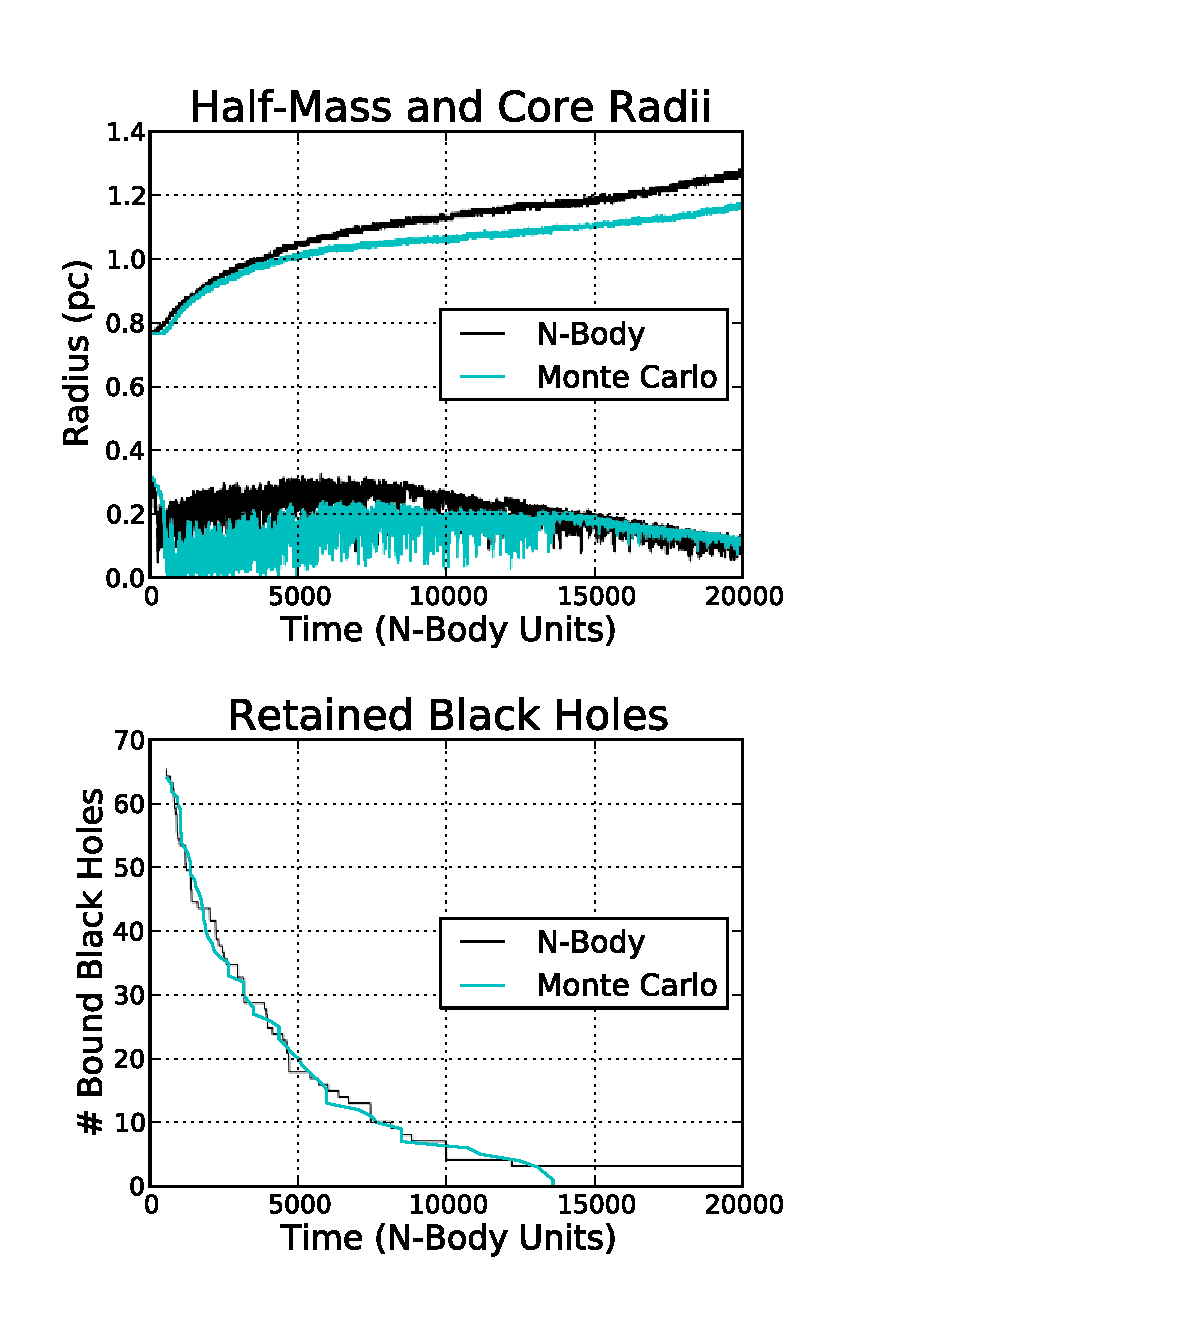
\includegraphics[scale=0.65]{64.pdf}
  \caption{Evolution of 2-Species Plummer models as computed by the Monte Carlo
  approach and the direct $N$-body approach of \cite{Breen2013}.  The
  top plot shows the half-mass radius (on top) and core radius (bottom) for the
  two methods, while the lower plot shows the number of retained BHs as
  a function of time.}
  \label{fig:2species64k}
\end{figure}


As in previous studies \citep{Joshi2000} we determine the optimal code
parameters by direct comparison to $N$-body simulations with identical initial
conditions.  Since the primary focus of this study is the retention of black holes,
we choose as our comparison an idealized two-component model recently studied 
in \cite{Breen2013} which provides a simplified description of the evolution of a population
of stellar-mass BHs in a cluster. These models are a realization of standard Plummer
sphere populated by a large population of low-mass stellar objects and a smaller
population of heavy objects.  We consider models with an individual mass ratio of
$m_2/m_1 = 20$, and a total cluster mass ratio of $M_2/M_1 = 0.02$, where $m_1$
and $m_2$ are the masses of individual particles, and $M_1$ and $M_2$ are the
total masses of each component.  We performed comparison simulations with $64k$ 
and $128k$ particles, although only the $64k$ runs are illustrated here.

In Fig. \ref{fig:2species64k}, we compare the cluster properties as reported by
the $N$-body simulations of \cite{Breen2013} to the results of our Monte
Carlo technique.  Empirically, we find optimal agreement by computing the
average quantities over the nearest 40 stars for two-body relaxation, and the
nearest 6 stars for three-body binary formation.  In particular, the 
evaporation rate of the black-hole subcluster in our simulations replicates
the $N$-body results extraordinarily well up to the ejection of the final
black-hole binary from the cluster.  Furthermore, we find the Monte Carlo
approach correctly reproduces the time evolution of the half-mass radius
to within 8\% after $2\times10^5$ $N$-body time units.  

Of the measured cluster properties, only the core radius cannot be
reproduced correctly by the Monte Carlo approach.  Immediately following core
collapse, the measured core radius for the Monte Carlo differs from the $N$-body
results by as much as 65\%.  Unfortunately this is to be expected: once mass
segregation and core collapse have occurred, the cluster core is comprised almost
entirely of black holes which have dynamically decoupled from the rest of the
cluster.  Correctly modeling the internal dynamics of an $N\sim100$ system using
a MC approach has very little hope of success; however, as the black holes are
ejected, and the core becomes populated with a larger number of lighter halo
stars, the validity of the MC approach is restored, and the core
radius better resembles that of the N-body approach.  Additionally, the core radius
is known to very sensitive to physical effects, such as three-body binary formation,
which is a stochastic process. New techniques are under
investigation that will correctly evolve the subcluster dynamics while
maintaining the speed of the MC approach. \textbf{For the present study,
we are encouraged by previous results from \cite{Morscher2013} suggesting
 that the BHs might actually never decouple from the cluster on the whole, 
 in which case a MC approach is appropriate.}



%%%%%%%%%%%%%%%%%%%%%%%%%%%%%%%%%%%%%%%%%%%%
%%%%%%%%%%%%%%%%                                             %%%%%%%%%%%%%%%%
%%%%%%%%%%%%%%%%                 INITIAL              %%%%%%%%%%%%%%%%
%%%%%%%%%%%%%%%%          CONDITIONS          %%%%%%%%%%%%%%%%
%%%%%%%%%%%%%%%%                                             %%%%%%%%%%%%%%%%
%%%%%%%%%%%%%%%%%%%%%%%%%%%%%%%%%%%%%%%%%%%%



\section{Initial Conditions}

We have calculated the dynamical evolution of 42 cluster models with a wide range of
initial conditions. All models are initialized as King models with stellar masses 
drawn from the \cite{Kroupa2001} initial mass function (IMF) from 
0.1 \,-\, 100$\, M_\odot$. We vary the initial number of stars 
($N=2 \times 10^5$, $8 \times 10^5$, and $1.6 \times 10^6$), the initial King 
concentration parameter ($W_o=2$, 5, 7) and the Galactocentric distance $R_G$, 
which in our models corresponds to three different metallicities
($Z=0.005$ at $R_G=2$ kpc, $Z = 0.001$ at $R_G\,=\,8$ kpc and $Z=0.0001$ at $R_G=20$ kpc). 
These initial conditions form a $3 \times 3 \times 3$ grid of 27 cluster models. 
Each of these models has initial virial radius $r_v\,=\,2$ pc and binary fraction
 $f_b = 10$\%. We will call these 27 models our \emph{standard models}.
 The choice to vary metallicity as a function of $R_G$ was 
 motivated by the currently observed properties of the Milky Way's GC population, 
 which show a correlation between $R_G$ and $Z$, with larger metallicities 
 corresponding to being found closer to the Galactic center \textbf{(ADD REF)}.

Beyond our standard models, we have run fifteen additional models
in which we have either varied a new parameter, or extended the range of one of the 
parameters from our $3\times3\times3$ sweep. For each $N$, starting with our 
intermediate parameters ($W_o$ = 5, $R_G$=8 kpc, $Z$=0.001),
we created models with larger central concentration ($W_o$ = 11), with smaller and
larger initial binary fraction ($f_b$ = 1\% and 50\%), and smaller and larger virial radius 
($r_v$ = 1 and 4 pc). We do not attempt to reproduce the distribution of GCs with 
different properties, but rather our goal is to see whether GCs with many BHs can 
evolve into $\sim 10\, \rm Gyr$ old clusters that are consistent with the properties of MW GCs. 
We evolve all of our models to a final time\footnote{Three of our low-$N$ models evaporated
before 12 Gyr, ending the simulation early} of 12 Gyr, which is a typical age for MW GCs. 
The properties of our initial models are given in Table \ref{table:initial_conditions}.


%\subsection{Initial Black Hole Populations}
For typical IMFs (e.g., Kroupa, Salpeter), a fraction of $\sim 10^{-4}\, - \,10^{-3} \, N$ \textbf{(update this)}
stars will become BHs. For our low-, intermediate- and large-$N$ models, 
we form $\approx 450$, 1750, and 3500 BHs, respectively. The initial BH mass spectrum
is shown for a subset of models in Figure \ref{fig:BHmasses}. 






%%%%%%%%%%%%%%%%%%%%%%%%%%%%%%%%%%%%%%%%%%%%
%%%%%%%%%%%%%%%%                                             %%%%%%%%%%%%%%%%
%%%%%%%%%%%%%%%%              RESULTS            %%%%%%%%%%%%%%%%
%%%%%%%%%%%%%%%%                                             %%%%%%%%%%%%%%%%
%%%%%%%%%%%%%%%%%%%%%%%%%%%%%%%%%%%%%%%%%%%%


\section{Results}

%\subsection{Description of Overall Evolution}
\subsection{Evolution of Clusters with Black Holes}

We start by describing the overall evolution of clusters containing many BHs, which 
is common to all of our models. The BHs form
within about 10 Myr and with masses $\sim 10$ times that that of typical stars, 
the BHs begin to sink due to dynamical friction against the light background stars. 
The timescale for segregation of the BHs from the half mass radius to the core is 
\begin{equation}
t_{seg} \sim \frac{\langle m \rangle}{M_{BH}} t_{rh}
\label{eq:segregation timescale}
\end{equation}
where $\langle m \rangle$ is the average stellar mass, $M_{BH}$ is the mass of the BH, 
and $t_{rh} \sim$ a Gyr is the half mass relaxation time. Since this timescale is dependent
on the $M_{BH}$, the heaviest BHs tend to sink to the core the fastest, driving a central collapse
(note: this is different from what is referred to as \emph{core collapse}, which occurs on a much longer
timescale). This can be seen in Figure \ref{fig:LagRad}, which shows the Lagrange radii
for a subset of 6 of our models (two for each $N$: \texttt{n2w5rg8, n2-D, n8w5rg8, n8-B, n16w7rg2 
and n16w7rg20}). By plotting the lagrange radii separately for the BHs (solid lines) 
and for the non-BHs (dotted lines), we see a clear separation of these two populations
over time, with the BHs becoming more centrally concentrated than lighter stars. 
Note that only a small subset ($\approx 1$\%) of the mass in BHs sinks \emph{deeply}, while the majority 
remains well mixed with the rest of the cluster. The collapse of the innermost BHs 
allows the core to reach high enough density that hard BH--BH binaries are formed
via three-body interactions. In this high density environment, these binaries, 
and potentially primordial binaries as well, experience strong binary interactions 
which can eject objects from the core or from the cluster entirely, while simultaneously injecting heat
into the cluster and powering a re-expansion. These core oscillations occur frequently
over the course of each simulation, as seen in Figure \ref{fig:LagRad}.

In Figure \ref{fig:potential} we zoom-in on one of the core oscillations in the lower right 
panel of Figure \ref{fig:LagRad} (model \texttt{n16w7rg20}) to show how the cluster potential
 fluctuates over a timescale of just a few Myr.
%In Figure \ref{fig:potential} we zoom-in on one of these early core oscillations for model 
%to show how the central gravitational potential of the cluster fluctuates 
%over the course of just a few Myr. 
During the collapse of the innermost $\approx 1$\% mass of BHs,
the BHs segregate from the lighter stars, forming \emph{temporarily} a cusp of mostly BHs. 
In the deepest part of the collapse, the central $\approx 30$ objects are all BHs. Several 
three-body binaries form during this phase (see top left panel) and their interactions
with other objects ultimately powers the re-expansion phase, which produces a BH 
core even larger in radius than it was pre-collapse. 
After the re-expansion, the BHs have become mixed in with the other stars once again. 
\textbf{(It would be interesting to see what determines exactly when the next BH collapse
will occur - is it when the last tight BH-BH is ejected? what is the role of primordial binaries?)}

In Figure \ref{fig:bhs_vs_time} we show the total number of BHs retained within 
each cluster model as a function of time. The abrupt increase in number of BHs within
$\approx 10$ Myr shows the period of BH formation. Soon after the BHs have segregated,
the number of retained BHs begins to decrease as BHs are ejected, and 
this continues through the end of each simulation. Since density increases with $N$, the 
larger-$N$ models have a higher rate of BH ejection, consistent with the higher rate
of strong binary encounters. Despite the higher ejection rate, however, these larger-N
models tend to retain a larger \emph{fraction} of BHs through 12 Gyr ($f_{ret,final}
 \approx 50$\%, compared to $\approx 20$\% for the lowest $N$ models).
This reflects the fact that models with larger $N$ are less dynamically 
evolved than those with lower $N$ after the same amount of physical time, since
their relaxation time is longer. 
The majority of our low-, intermediate-, and high-$N$ models end with $\approx 50-100$ BHs,
$\approx 400-800$ BHs, and $\approx 1000-2000$ BHs, respectively, but the smallest number
of retained BHs in any model is 9. Across all models, most of the retained BHs are \emph{single} objects. 

In Figure \ref{fig:CumBinintEscBHs} we show the evolution of the total number of binary-binary
(B-B) and binary-single (B-S) interactions along with the total number of ejected single BHs, 
BH-BH binaries, and BH-non-BH binaries, for the same six models shown in Figure \ref{fig:LagRad}.
 The early phase of rapid 
BH ejection represents BHs that are ejected at birth via supernova kicks prior to 10 Myr, 
and is followed by a flattening of the BH ejection rate, during which time the BHs
are segregating. By around 100 Myr, the binary 
interaction rate increases abruptly, and with it comes an increase in the BH ejection 
rate. In particular, the BH-BH ejection rate seems to be most sensitive to the B-B 
interaction rate. This is to be expected, since in a B-S interaction, assuming three stars of
comparable mass, it is much more probably that the \emph{single} star will be 
ejected than the \emph{binary}. Hard binaries that experience multiple encounters
can become tight enough that the recoil kick on the binary is sufficient to eject
it from the cluster. The binaries that are ejected, therefore, are most often BH-BH 
binaries, since encounters should tend to replace any lighter non-BH binary 
companions with the heavier BHs in 
the process. We find that the number of ejected BH-BH binaries is typically
more than an order of magnitude larger than the number of ejected BH-binaries with a 
non-BH companion. 


Figure \ref{fig:mass_evolution} 
shows the evolution of total cluster mass for all 42 models.  Within the first 
few Myr, there is a phase of rapid mass loss from stellar evolution. After the most massive 
stars have evolved, the rate of mass loss slows to a nearly steady rate and is due to both 
tidal stripping and stars becoming gravitationally unbound by obtaining a velocity above
the cluster escape velocity. Most of our models lose about half of their mass by 12 Gyr. 
It is well known that clusters lose significant amount of their mass over Gyr timescales, which
is why the smallest clusters have already evaporated, and also why we must initialize
our models with at least twice the mass we wish to have at the end of the simulation.
In fact, our three models with $N=2 \times 10^5$ and the smallest  $R_G$ 
(\texttt{n2w5rg2, n2w5rg2, n2w7rg2}) evaporate due to the tidal effect of the 
Galaxy within 6 Gyr (dotted lines in the upper
left panel of Figure \ref{fig:mass_evolution}). 

In general, we find that the final cluster mass is directly proportional to $R_G$, as would be
expected. However, the models with $R_G$ of either 8  or 20 kpc tend to lose mass at a similar rate.
In addition to $R_G$, the initial virial radius also affects the cluster mass loss significantly, 
especially for small $N$ models, which have shorter relaxation times, and thus are dynamically
older than larger $N$ models at 12 Gyr. For example, model \texttt{n2-B} with $N=2 \times 10^5$ and 
$r_v=1$ pc loses more than 80\% of its mass by the end of the simulation.  


 %%%%%%%%%%%%%%%%%%%%%%%%%%%%%%%%%%%%%%%%%%%%
%%%%%%%%%%%%%%%%                                             %%%%%%%%%%%%%%%%
%%%%%%%%%%%%%%%%           ANALYSIS              %%%%%%%%%%%%%%%%
%%%%%%%%%%%%%%%%              OF   BHs               %%%%%%%%%%%%%%%%
%%%%%%%%%%%%%%%%                                             %%%%%%%%%%%%%%%%
%%%%%%%%%%%%%%%%%%%%%%%%%%%%%%%%%%%%%%%%%%%%

\subsection{Analysis of BH-Binary Populations}

Next we look at the properties and evolution of the BHs in more detail.
The final BH mass distribution for the same six models is shown in Figure \ref{fig:BHmasses}
along with the mass distribution soon after the BHs are formed. Since the heaviest BHs 
(at any given time) are most likely to be found in the dense core region where they can 
participate in binary interactions.We find that the heaviest BHs
are ejected first, which is a consequence ofthe fact that these  Over time,
the maximum BH mass in the cluster is reduced from $\approx 25-30 M_\odot$ down to 
$\approx 15-20 M_\odot$. Thus, even at 12 Gyr, many of our models still contain a
substantial population of 10$M_\odot$ BHs.

The overall populations of retained and ejected BHs for each model are shown in 
Table \ref{table:bhs}. As mentioned previously, most of the retained BHs
remain as single stars throughout the cluster evolution, with at most
tens of BH-binaries (of any type) in the cluster at any given time, and often fewer than ten. Of these binaries, 
there are typically a comparable number of BH-BH binaries and BH-non-BH binaries.
There are a handful of BH-WD binaries across the set of models, but BH-NS
binaries are virtually nonexistent. For models with 
large-$N$ and binary fractions of $f_b=50$\% 
have significantly more BHs in binaries than models with lower $f_b$. For example
in the $N= 1.6 \times 10^6$ model with $f_b$=50\%, the number of BH binaries (of any type)
can be from about 3-8 times larger than the other models with the same $N$ but 
lower binary fractions (depending on other parameters). This indicates that it is not 
only three-body binaries formed in the 
core that involve BHs, but rather, a larger population of binaries provides more 
opportunity for BHs to exchange into a binary system.

Systems with smaller initial virial radii tend to eject BHs at a higher rate due to
the increased density, and thus end with significantly fewer
BHs (yellow curves on right panels of Figure \ref{fig:bhs_vs_time}), and the opposite is true for 
models with larger initial virial radius (blue curves on the same panels). We find that the models 
with smaller $R_G$ retain fewer BHs
at 12 Gyr, but this is mostly a reflection of the fact that they were not able to retain as many BHs
initially due to their smaller tidal radii. Figure \ref{fig:RetBHsSingleBinary}
shows the distribution of single versus binary BHs within a subset of models. 
%Across all simulations, the majority of BHs present in the cluster are \emph{single}, 
\textbf{.......TO DO:  Finish describing the details of the BH population, e.g., single vs binary, and
describe ejected BH sources, connection to binary interaction rate, etc.}

Our models produce a large number of BH-BH mergers




%%%%%%%%%%%%%%%%%%%%%%%%%%%%%%%%%%%%%%%%%%%%
%%%%%%%%%%%%%%%%                                             %%%%%%%%%%%%%%%%
%%%%%%%%%%%%%%%%           OBSERVABLE       %%%%%%%%%%%%%%%%
%%%%%%%%%%%%%%%%           PROPERTIES         %%%%%%%%%%%%%%%%                                      
%%%%%%%%%%%%%%%%                                             %%%%%%%%%%%%%%%%
%%%%%%%%%%%%%%%%%%%%%%%%%%%%%%%%%%%%%%%%%%%%


\subsection{Observable Properties: Comparison to Galactic GCs}

In order to know whether our models are a good representation of reality we must
calculate observable properties for our models and compare them to those of real
GCs. Among these key observable properties are the core radius ($r_c$), the ratio of the 
core radius to the half-light radius ($r_c / r_h$), the central (3D) luminosity 
density ($\rho_0$) and total cluster mass ($M_{cl}$). We calculate these four values
for each of our models at the final time of 12 Gyr, with the exception of the three models that evaporated
 prior to 12 Gyr.
 
Since the cluster mass is a straightforward quantity in our models, here we do the simplest 
thing and report our theoretical total cluster mass, which is the sum of the masses of all the individual stars, 
including dark remnants. The other three quantities are less straightforward, and so we must do a bit more work to obtain values that can reasonably be compared to the ones that observers would actually calculate. Since observations of GCs are generally in the $V$-band, we start by converting the bolometric luminosity for each star as given by BSE to $V$-band luminosities using the standard stellar library of \cite{Lejeune1998}. From there, the half-mass radius $r_h$ is simply the radius that encloses half of the light (in the $V$-band).
The core radius of a GC is a quantity that has produced a great deal of confusion in the literature (REF) because there are many different definitions, and the resulting value can vary by a factor of a few depending on which one is being used. Qualitatively, the core of a cluster is the central region over which the density and velocity dispersion are roughly constant. 
More quantitatively, the core radius is sometimes defined as the radius at which the surface luminosity density
drops to half the central value. To calculate $r_c$, observers generally make a surface brightness 
profile (SBP), and then measure where the density drops to half the central value. Alternatively, a King model can be fit directly to 
the SBP. To make an SBP requires the stars to be binned radially. The bins should be small enough in radius that the core is resolved. The tradeoff is that small bin sizes increase the random noise, since a single bright star can dominate the light
for an individual bin, introducing large bin-to-bin variations. To get around this observers generally remove the brightest stars
before calculating the SBP \citep{Noyola2006} based on a somewhat arbitrary choice of a magnitude cutoff. A detailed discussion and comparison of these various techniques can be found in \cite{Noyola2006}. In this work, we have instead opted to use a new approach for calculating $r_c$ that eliminates the need for binning, as well as the complications that go along with it. Our method relies on the \emph{cumulative} luminosity profile, to which we fit the integrated form of a King density profile, and extract the best fit value of $r_c$. We find that this function provides an excellent fit to our models' integrated light profile. For comparison, we have also calculated $r_c$ from the SBP  for our models using a technique similar to \cite{Noyola2006}, and find that the two techniques produce reasonable agreement. 
With our computed values of $r_c$, we calculate the central 3D luminosity density, $\rho_{l,x}$ (in units of $L_{\odot,x}/pc^3$) 
within both $0.1\, r_c$ and $0.25\, r_c$.

%The core radii determined with our new method agreed to within ~blah percent of the values based on the SBP. 

Using the calculated core radii, we calculate the 3D central luminosity density, $\rho_{l,x}$ (in units of $L_{\odot,x}/pc^3$) within $0.1\,r_{c,x}$, where $x$ designates whether the bolometric ($b$) or the visual ($v$) luminosities are used in the calculation.
\textbf{TO DO: add the equation}. The half-light radius, $r_{h,x}$, is simply the radius that encloses half of the total cluster luminosity. The observable properties are shown in Table \ref{table:Observables}.


\subsection{Comparison to Galactic GCs}


In Figure \ref{fig:MW_histograms} we compare $r_c$, $r_c / r_h$, $\rho_c$, and $M_{tot}$ 
for our models to the actual values observed in MW GCs. All the Galactic GC data is taken
from the \cite{Harris1996} catalog (2010 edition), except for the total 
cluster mass, which is taken from \cite{Gnedin1997}. The true properties of MW 
GCs are represented as histograms, and the colored tick marks indicate the final values for our 
models. Our $N=8 \times 10^5$ runs produce final clusters with roughly around the median GC mass of about $10^5\, M_\odot$. With our three different values of $N$, our final cluster masses span most of the range of
MW GC masses. To model the largest MW clusters, we will have to extend our initial $N$ to larger values.

While the masses and densities of our models agree well with the 
distribution of MW GCs, we have a deficit of models with small values of $r_c$ and $r_c / r_h$. 
Most MW GCs have a core radius less than 1 pc, however only one of our models has falls under
a pc (our lowest-$N$ model with reduced $R_v=1$ pc, which has $r_c=0.5$ pc at 12 Gyr). 
Our models do, however, produce core radii that fall within the region covered by the MW GCs,
although the bulk of our models have $r_c$ of $\approx 2-4$ pc.

The presence of large populations of BHs throughout the evolution of our models
produces a continuous heat source that prevents the cores in our models from
contracting. The only model to reach a sub-parsec core size is a low-$N$ model with
$r_v=1$ pc, which is able to eject nearly all of its BHs, with only 9 remaining at 12 Gyr.


%%%%%%%%%%%%%%%%%%%%%%%%%%%%%%%%%%%%%%%%%%%%
%%%%%%%%%%%%%%%%                                             %%%%%%%%%%%%%%%%
%%%%%%%%%%%%%%%%           DISCUSSION         %%%%%%%%%%%%%%%%
%%%%%%%%%%%%%%%%                                             %%%%%%%%%%%%%%%%
%%%%%%%%%%%%%%%%%%%%%%%%%%%%%%%%%%%%%%%%%%%%




%\subsection{BH Mergers}
%1. Discuss overall numbers and properties of mergers inside and outside of clusters
%
%2. Compare models: which had highest merger rate and why?
%
%3. Combined merger rate: decide on simple technique for combining simulations. Provide rate per Milky Way Equivalent Galaxy (MWEG); compare to pop. synth. estimates for field
%
%4. Figure: histogram of MW clusters, binned according to our model values, for M and rc/rh.  Well, maybe I won't show this?
%
%5. For one model, show number of mergers binned over time.
%
%6. Figure: Histogram of chirp masses at different times, (one curve represents mergers up to 6 Gyr, another curve represents distribution of mergers over the entire 12 Gyr)....there should be some dependence of average chirp mass as a function of time.



\section{Conclusions}






%%%%%%%%%%%%%%%%%%%%%%%%%%%%%%%%%%%%%%%%%%%%%
%%%%%%%%%%%%%%%%                                        %%%%%%%%%%%%%%%%%%
%%%%%%%%%%%%%%%%           FIGURES           %%%%%%%%%%%%%%%%%%
%%%%%%%%%%%%%%%%                                        %%%%%%%%%%%%%%%%%%
%%%%%%%%%%%%%%%%%%%%%%%%%%%%%%%%%%%%%%%%%%%%%



%=======================================================================
%====================     							            ===================
%====================    		    LAGRANGE    RADII       	   ===================
%====================     							            ===================
%=======================================================================

%---------   Lagrange Radii plots -------------

\begin{figure}[!h]
\epsscale{0.8}
	\plotone{bh_lagrad_6models.eps}
	% MAKE THIS FIGURE: from 3x3x3 directory
	% >>> extract_model_details.plot_multiple_panels(plotbinint=1,plotretbhs=1,plotdensity=1,plotlagrad=1)
	\caption{Evolution of the Lagrange radii for a subset of models, calculated separately 
	for the BHs (\emph{solid lines}) and for other objects (\emph{dotted lines}). The Lagrange
	radii shown enclose a fixed fraction of the mass (\emph{from bottom to top}) of 0.1\%, 1\%, 
	10\%, 50\% and 90\%, for each individual component (BHs, non-BHs). The six models shown 
	are as follows. \emph{Top left}:  \texttt{n2w5rg8} ($N=2 \times 10^5$, $W_o=5$,  $r_v=2$ pc, 
	$R_G=8$ kpc, $Z=0.001$, and $f_b=10$\%). \emph{Top right}: \texttt{n2-E} (same as left, but 
	with larger binary fraction $f_b=50$\%). \emph{Center left}: \texttt{n8w5rg8} ($N=8 \times 10^5$, 
	$W_o=5$, $r_v=2$ pc, $R_G=8$ kpc, $Z=0.001$ and $f_b=10$\%). Center right: \texttt{n8-B} (same 
	as left, but with smaller virial radius $r_v=1$ pc). \emph{Bottom left}:  \texttt{n16w7rg2} 
	($N=1.6 \times 10^6$, $W_o=7$, $r_v=2$ pc,  $R_G=2$ kpc, $Z=0.005$, and $f_b=10$\%). 
	 \emph{Bottom right}: n16w7rg20 (same as left, except $R_G$=20 kpc and $Z=0.0005$).
	For all models, within $\approx 200$ Myr the heaviest BHs, which segregate the fastest, 
	drive a central collapse of the innermost $\approx 1$\% of  BH mass. The rest of the BH mass 
	follows, segregating on a slightly longer timescale, but not nearly as deeply as the central 1\%, while the rest of
	the cluster steadily expands. By about a Gyr (even sooner for the lower-$N$ models), the 90\% BH Lagrange 
	radius (\emph{solid magenta line}) coincides with the 10\% Lagrange radius of the rest of the cluster 
	(\emph{dotted red line}). Over time, the BHs continue to segregate while the rest of the cluster 
	expands until more than 90\% of the BH mass is confined to a region containing less than 10\% of 
	the rest of the cluster. However, by 12 Gyr most of our models have masses of $\approx 5 \times 10^4-
	5 \times 10^5 M_\odot$, and so the remaining $\sim 100-1000$ BHs are well
	mixed with a significant number ($\sim 10^3-10^4$) of other stars. 
	For some of our models, the early output frequency was too low and the
	initial phase of BH contraction was not captured.
	}
	
	\label{fig:LagRad}
\end{figure}


\begin{figure}[!h]
\epsscale{0.8}
	\plotone{3panel_potential_plot_r36.eps}
	\caption{Time variation of central gravitational potential through a period of collapse and re-expansion 
	for model with $N=1.6 \times 10^6$, $W_o=7$, $r_v=2$ pc, $R_G=20$ kpc, $Z=0.005$, and $f_b=10$\%, 
	(\emph{bottom right} panel in Figure \ref{fig:LagRad}) around 200 Myr. \emph{Top left}: zoom in of the 
	Lagrange radii from about 180--220 Myr, which shows a deep collapse and re-expansion of the central BHs.
	The radial coordinate is given in units of the initial half-mass radius ($r_h$(0)). The 
	three solid curves are the 0.1\%, 1\% and 10\% Lagrange radii of the BHs, and the dotted curve is the 0.1\%
	Lagrange radius for the non-BHs. The vertical dashed lines indicate the time of formation
	of three-body binaries. During each of these collapses, tight three-body binaries form and begin
	to interact with other single and binary objects, injecting heat into the system. We study the potential
	over the period spanned by the vertical solid red lines on the right and the bottom panels.
	\emph{Top right}: the full gravitational potential profile, $\phi(r)$, at four different times 
	(as indicated on the bottom panel), in units of $G\, M / r_h$, where M is the
	total cluster mass and $r_h$ is the half-mass radius, at the given time. Beyond $r\approx10^{-1}\,r_h$,
	the cluster potential is fixed over this period of a few Myr. Within that radius, however, the potential
	fluctuates significantly over this short timescale, forming a central cusp at the most contracted phase.
	\emph{Bottom}: zoom-in on the central region of the potential. The times of each potential curve are 
	indicated on the figure. The ticks on the curves indicate the radial positions of the innermost 50 BHs
	(red) and innermost 50 non-BHs (blue), at each time. The central part of the cluster starts at a 
	relatively expanded phase at 201.3 Myr (second from the top) and then collapses 
	(bottom two curves), before re-expanding more dramatically (top curve). The position of the innermost
	object varies by more than an order of magnitude between the collapsed and expanded 
	phase. During the collapsed phase, the central region is dominated by a cusp of BHs, with 
	the first non-BH objects sitting outside of about 30 BHs. In the expanded phases, 
	the BHs and stars become well-mixed once again.
	}
	\label{fig:potential}
\end{figure}

%=======================================================================
%====================     							            ===================
%====================    		   NUMBER  OF  BHs             	   ===================
%====================     			  VS   TIME		            ===================
%====================     							            ===================
%=======================================================================

\begin{figure}[!h]
\epsscale{1.0}

	\plotone{ret_bh_time_evol_logy.eps}  
                % MAKE THIS FIGURE:  from 3x3x3 directory, run
                % >>> extract_model_details.plot_time_evol_multipanel('.bhs.dat', cols=[2,], ylabel=''number of black holes')
	\caption{Total number of retained BHs as a function of time, for all models.
	 From top to bottom, the pairs of panels shows all models with $N=2 \times 10^5$, 
	 $N=8 \times 10^5$ , $N=1.6 \times 10^6$. On the left three panels, we show the nine 
	 standard models at each $N$, and on the right three panels we show the five additional 
	 models at each $N$. For the left panels, the different colors indicate the initial central 
	 concentration ($W_o=2$ in black, $W_o=5$ in red, and $W_o=7$ in blue), the different
	 lifestyles indicate the initial galactocentric distance and metallicity (solid lines have 
	 $R_G=20$ kpc and $Z=0.0005$, dashed lines have $R_G=8$ kpc and $Z=0.001$,
	 and dotted lines have $R_G=2$ kpc and $Z=0.005$. All of these models have 
	 $R_v=2$ pc and $f_b=10$\%. On the top left, the three models with smallest $R_G$ 
	 (dotted lines) evaporated prior to 12 Gyr, at which point the runs were halted.
	 For the panels on the right, the
	 black dashed lines show (for comparison) the standard model from the corresponding
	 left panel with intermediate parameters (i.e., $W_o=5$, $R_G=20$ kpc, $Z=0.0005$, 
	 $r_v=2$ pc, $f_b=10$\%), for each $N$. Each of the solid colored lines has one parameter 
	 slightly different from this intermediate model: in red we show the models with the highest 
	 concentration ($W_o=11$), in yellow and blue the models with smaller and larger 
	 initial virial radius ($r_v = 1, 4$ pc) respectively, and in green and cyan the models 
	 with lower and higher binary fraction (($f_b=1$\%, 50\%) respectively. As can be seen
	 in these panels, the initial virial radius has the greatest impact on BH retention, with
	 the models with $r_v=1$ pc (yellow) retaining a significantly lower number of
	 BHs at 12 Gyr than those with $r_v=4$ pc (blue). The lowest-$N$ model has just nine 
	 BHs remaining at the end of the simulation.}

	\label{fig:bhs_vs_time}
\end{figure}





%=======================================================================
%====================     							            ===================
%====================    		     BIN INTs + ESC BHs   	         	  ===================
%====================     							            ===================
%=======================================================================

\begin{figure}[!h]
\epsscale{1.0}
	\plotone{cum_binint_escbhs_6models.eps}
	% MAKE THIS FIGURE: from 3x3x3 directory
	% >>> extract_model_details.plot_multiple_panels('.bin.dat', [0,8,9], ['BB','BS'],'log(time) (Gyr)', 'cumulative number')
	\caption{Cumulative number of binary interactions and ejected BHs as a function of time for the 
	same six models as described in Figure \ref{fig:LagRad}. Black dashed and dotted curves show 
	the cumulative number of binary-binary (B-B) and binary-single (B-S) interactions over time. 
	The solid curves show the cumulative number of ejected single BHs (red),
	BH-BH binaries (blue), and BH-other binaries (cyan) as  function of time. Central density increases
	with increasing $N$ (top to bottom), and as a result, binary interactions tend to become important 
	earlier for larger-$N$ models. Models with just 10\% binaries (all except the top right panel),
	have significantly more B-S interactions than there are B-B interactions, as there are so many 
	more single stars than binaries. The model shown in the top right panel has $f_b=50$\% 
	(equal number of single and binary objects), and hence has a comparable B-S and B-B interaction rate.
	The jump in ejected BHs occurring around 10 Myr reflects BHs that are ejected at time of
	formation due to supernova kicks. In many models, we see an increase in the B-B ejection rate
	after about 100 Myr, which also corresponds to an increase in the BH-BH ejection rate.
	Very few, if any, binaries containing a BH with a non-BH companion are dynamically ejected, 
	since they are short-lived compared to BH-BH binaries. Among those that are ejected, 
	nearly all have stellar companions (rather then non-BH remnants). The dominant population
	of ejected BH binaries are BH-BH binaries. 
	}
	
	\label{fig:CumBinintEscBHs}
\end{figure}

%=======================================================================
%====================     							            ===================
%====================    		     CLUSTER MASS             	   ===================
%====================     			  VS   TIME		            ===================
%====================     							            ===================
%=======================================================================


\begin{figure}[!h]
\epsscale{0.8}
	\plotone{mass_time_evolution.eps}
	% MAKE THIS FIGURE: from 3x3x3 directory
	% >>> extract_model_details.plot_time_evol_multipanel(fileending='.dyn.dat', cols=[4,], y='mass',ylabel='M$_\mathrm{cl}$ ($10^5$ M$_\odot$)')
	\caption{Evolution of the total cluster mass for all models. The different line colors and styles are 
	described in Figure \ref{fig:bhs_vs_time}. \textbf{Add the rest of this caption}. 
	}
	
%	Models:  From top to bottom, we show models with initial $N=2 \times 10^5$, $N=8 \times 10^5$ and $N=1.6 \times 10^6$. In the panels on the left, the black, red and blue lines show models with initial $W_o=2$, $W_o=5$ and $W_o=7$, respectively. The solid, dashed and dotted lines show models with initial $R_G=20$ kpc, $R_G=8$ kpc and $R_G=2$ kpc, respectively. For the panels on the right, the red line is for the model with the highest concentration ($W_o=11$), yellow and blue show the models with smaller and larger initial virial radius ($r_v = 1, 4$ pc), and green and cyan show the models with lower binary fraction ($f_b=1$\%) and higher binary fraction ($f_b=50$\%). For comparison, the black dashed line shows the intermediate model from the $3 \times 3 \times 3$ grid ($W_o=5$, $R_G=8$ kpc, $r_v=2$, $f_b=10$\%, for each $N$).
	
	\label{fig:mass_evolution}
\end{figure}




%=======================================================================
%====================     							            ===================
%====================    		     BH  MASS  SPECTRA       	   ===================
%====================     							            ===================
%=======================================================================

\begin{figure}[!ht]
\epsscale{0.8}

	\plotone{bh_mass_functions_6models.eps}

	\caption{BH mass spectrum at a time soon after the BHs are formed (solid black lines) 
	and at 12 Gyr (dashed grey lines) for the same six models described in Figure \ref{fig:LagRad}.
 	In all models, the heaviest BHs are the first to be ejected because they segregate more deeply 
	than the lighter BHs, and therefore have the highest interaction rate. By the end of the simulation,
  	the maximum BH mass has dropped from more than $25\,M_\odot$ down to $\approx 15-20\,M_\odot$, 
	depending on the model. In general, the lower-$N$ models tend to eject a higher fraction of 
	their BHs. The parameter that has the greatest impact on the initial BH population is the metallicity $Z$.
	All models shown have $Z=0.001$ (with corresponding $R_G=8$ kpc) except for the one shown
	In the lower left panel, which has $Z=0.005$ (with $R_G=2$ kpc), the largest metallicity used in this work. Higher metallicity
	stars experience greater wind mass loss rates and end up with lower core masses, which in turn
	produces less massive remnants. This explains the pileup of BHs at about $20\,M_\odot$, which results
	from a flattening of the progenitor-to-remnant mass relation (see Figure 1 of \cite{Belczynski2004}).
	}
%top left: 		n2e5w2r2Rg8z0.001fb10
%top right: 		n2e5w5r2Rg8z0.001fb50
%center left:		n8e5w5r2Rg8z0.001fb10
%center right:	n8e5w5r1Rg8z0.001fb10
%bottom left:	n1.6e6w7r2Rg2z0.005fb10
%botom right:	n1.6e6w7r2Rg20z0.0005fb0.1
	\label{fig:BHmasses}
\end{figure}



%=======================================================================
%====================     							            ===================
%====================    		     RET BHs:                         	   ===================
%====================     		single vs  binary		            ===================
%====================     							            ===================
%=======================================================================

	\begin{figure}[!h]
\epsscale{1.0}
	\plotone{ret_bh_time_evol_details_6models.eps}
	%\plotone{bh_ret_single_binary_time_evol_6models.eps}

	\caption{More detailed look at the retained BH populations for the same six models as
	described in Figure \ref{fig:LagRad}. Here we show the numbers
	of retained single and binary BHs as a function of time. The single BHs are shown in red, the 
	BH-BH binaries are in blue, and the BH binaries with non-BH companions (BH-other) are in
	cyan. An initial population of as many as tens of primordial BH binaries with non-BH companions is 
	reduced very quickly, since lighter stars in binaries tend to be replaced by heavy BHs through 
	dynamical interactions. For all models, however, nearly all retained BHs are single throughout 
	the entire 12 Gyr evolution. This is due to the fact that only the innermost few percent of BHs 
	are found in the dense core where binary interactions are occurring frequently, and therefore only this subset of
	BHs is able to exchange into binaries. Comparing the two $N=2 \times 10^5$ models on the top, the model on
	the right, which has a larger binary fraction ($f_b=50$\%) than the model on the left ($f_b=10$\%)
	has a larger population of BH-other binaries at most times, but similar number of BH-BH binaries
	(except during the first few 100 Myr). For the two plots in the middle, which have $N=9 \times 10^5$
	stars initially, but different $r_v$ (2 pc on the left, 1 pc on the right), the retained BH populations
	are similar, except the model with smaller $r_v$ loses more BHs. The panels on the bottom
	both have $N=1.6 \times 10^6$ stars, and differ in $R_G$ and Z (left panel has smaller $R_G$
	and larger $Z$),  and evolve similarly except the higher $Z$ model ends with fewer BHs.
	}
	
	\label{fig:RetBHsSingleBinary}
\end{figure}



\begin{figure}[!ht]

	\plotone{bh_binary_properties_by_N.eps}
	% >>>  extract_model_details.plot_bh_binary_properties(col='n',value=16, plotmarker='.',marker_size=2, marker_face_color='k', plotcolor='k')
	% >>>  extract_model_details.plot_bh_binary_properties(col='n',value=8, plotmarker='.',marker_size=1.5, marker_face_color='c', plotcolor='c')
	% >>>  extract_model_details.plot_bh_binary_properties(col='n',value=2, plotmarker='.',marker_size=1.5, marker_face_color='r', plotcolor='r')

	
	\caption{Properties of ejected BH-binaries from all simulations. The first two panels show properties of ejected 
	the $\approx 5600$ BH-BH binaries ejected from all models combined.
	On the left we plot $m_2$ versus $m_1$ for all BH-BH binaries, and in the middle the semi-major axis versus the eccentricity 
	for the same binaries. For ejected binaries containing a BH and a non-compact star, we show the semi-major axis versus the 
	mass of the stellar companion. The color of the point indicates the initial $N$ for the cluster from which the binary originated
	(black for $N=1.6 \times 10^6$, cyan for $N=8 \times 10^5$, and red for for $N=2 \times 10^5$. While the larger-$N$ models
	eject more BH-BH binaries, the masses of the binary components ejected are similar across all $N$. There is larger number
	of ejected binaries with both BH components of mass of about 20 $M_\odot$, since these are always the first to be ejected, and
	there remain many lower-mass BHs that are retained in the models. The orbital properties of ejected BH-BH binaries does 
	depend on $N$, with lowest-$N$ clusters ejecting binaries with significantly lower semi-major axes (typically $\sim 1$ AU) 
	than the largest-$N$ clusters (typically $\sim 0.1$ AU). This is because it is easier to eject a binary from a lower-$N$ model
	due to its lower escape speed, and so most of these BH-BH binaries are ejected before they have a chance to get down 
	to sub-AU separations.
	On the right panel we show the semi-major axis and the companion mass for the 227 ejected binaries containing a BH with a non-compact
	stellar companion. The lower-$N$ models eject fewer binaries with heavy companions because...?
	Note that there there is a great
	deal of overlap between the the points for the three different $N$ values, and so many of the black points are covered by the cyan
	and red points, which are plotted on top of the black.
	points are covered by
	}
	\label{fig:bh_binary_properties}
\end{figure}




%=======================================================================
%====================     							            ===================
%====================    		     COMPARISON TO	        	   ===================
%====================     		       GALACTIC  GCS 	            ===================
%====================     							            ===================
%=======================================================================


\begin{figure} [!ht]
\epsscale{1.0}

	\plotone{mw_gcs_models_comparison.eps}  
	% To make this figure, from directory with tables (final_properties.dat, my_gc_table_rc_pc.dat)
	%  >>>     extract_model_details.make_MW_histograms()
	\caption{Comparison of observable properties for MW GCs and for our models. The MW data is taken from the \citealt{Harris1996} (2010 edition), excluding the masses, which are from \citealt{Gnedin1997}. The histograms show the distribution of core radii, $r_c$, the ratio of core to half light radius, $r_c\, /\, r_h$, the central luminosity density, $\rho_c$, and total cluster mass, $M$, for the Milky Way GCs (Harris). The ticks show the calculated values for the same quantities for our models. The colors indicate the initial value of $N$. For quantities that depend on \emph{light} (all of the above, except for $M$), we have calculated the quantities with at least two different methods, which are represented by the different sets of ticks at the bottom, center, or top of the plots. For $r_c$ and $r_h$, the ticks on the bottom and top are calculated using the cumulative luminosity function using visual or bolometric luminosities, respectively. The ticks across the middle of the plot of $r_c$ show the values as calculated from the surface brightness profile. For and $\rho$, the bottom set of ticks shows the luminosity density calculated in the visual band within either 0.1 $r_c$ or 0.25 $r_c$, and the two sets of ticks at the top of the panel represent the same quantities as derived from the bolometric luminosities. $M$ is simply the sum of all the masses in the cluster. Our clusters agree well with MW GCs in terms of $\rho_c$ and $M$, but our measured values for $r_c$ and $r_c / r_h$ fall on the high end of the distribution. The three low-$N$ models that dissolved prior to 12 Gyr are excluded from these figures.}

	\label{fig:MW_histograms}
\end{figure}






%=======================================================================
%====================     							            ===================
%====================    			FLUCTUATIONS        	   ===================
%====================     		       REPEATED RUNS 	            ===================
%====================     							            ===================
%=======================================================================


% ---------------------------------------     Mass vs Time,   BHs vs Time,         -----------------------------------

%\begin{figure}
%	\centering
%       
%        \begin{subfigure}[b]{0.45\textwidth}
%                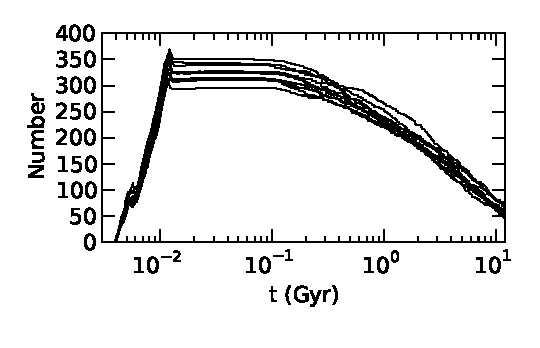
\includegraphics[width=\textwidth]{r5_repeat10_bh_ret_timevolution.eps}
%
%                \label{fig:repeat10_bhs}
%        \end{subfigure}     
%        \begin{subfigure}[b]{0.5\textwidth}
%                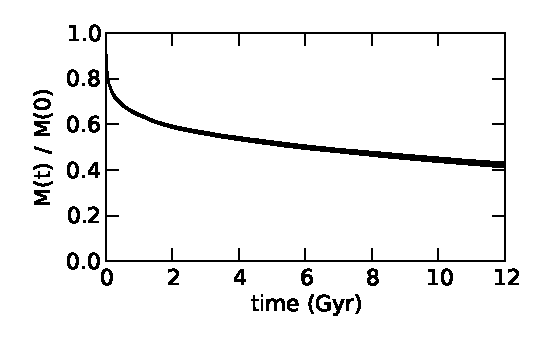
\includegraphics[width=\textwidth]{r5_repeat10_mass_timeevolution.eps}
%                \label{fig:repeat10_mass}
%        \end{subfigure}     
%
%
%	\caption{S\textbf{I have not completed this figure/analysis yet} Statistical fluctuations across 10 realizations of one cluster model - model r5. The total cluster mass, number of BHs as a function of time agree very well across all 10 simulations. \bf{TO DO: plot rc and rh as a function of time for all models - run script over all snapshots}}
%
%\end{figure}




%\begin{figure}[!h]
%\epsscale{1.0}
%
%	\plotone{mw_rc_vs_M_comparison.eps}
%
%	\caption{$}
%	\label{fig:MW_models_Rc_vs_M}
%\end{figure}

       



%%%%%%%%%%%%%%%%               TABLES           %%%%%%%%%%%%%%%%%





%%%%%%%%%%%%%%%%%%%%%%%%%%%%%%%%%%%%%%%%%%%%
%%%%%%%%%%%%%%%%                                             %%%%%%%%%%%%%%%%
%%%%%%%%%%%%%%%%              IC  TABLE            %%%%%%%%%%%%%%%%
%%%%%%%%%%%%%%%%                                             %%%%%%%%%%%%%%%%
%%%%%%%%%%%%%%%%%%%%%%%%%%%%%%%%%%%%%%%%%%%%


\begin{deluxetable}{lccccclcccc}
%\tablecolumns{7}
\tabletypesize{\tiny}
%\tablewidth{0pc}
\tablecaption{Initial model parameters.}

\tablehead{
	\colhead{model} & \colhead{$N$} & \colhead{$M$} & \colhead{$W_0$} & \colhead{$r_v$} & \colhead{$R_G$} & \colhead{$Z$} & \colhead{$f_b$} & \colhead{$r_{c,code}$} & \colhead{$r_{h,code}$} & \colhead{$log(\rho_{c})$}   \\
\colhead{} & \colhead{$(10^5)$} & \colhead{$(10^5 M_{\odot})$} & \colhead{} & \colhead{pc} & \colhead{(kpc)} & \colhead{} &  \colhead{\%} &\colhead{(pc)} &  \colhead{(pc)}  & \colhead{$(M_{\odot}$/pc$^3)$}
}

\startdata
%#1:model  #2:N,i/1e5  #3:M,i/1e5  #4:Wo  #5:rv(pc)  #6:Rg(kpc)  #7:Z  #8:fb(%)  #9:rc_theor,i  #10:rh_theor,i  #11:log10(rho_c,i)
n2w2rg2		& 2	& 1.36	& 2	& 2	& 2	& 0.005	& 10	& 1.0	& 1.7	& 4.47 \\ 
n2w2rg8		& 2	& 1.36	& 2	& 2	& 8	& 0.001	& 10	& 1.0	& 1.7	& 4.47 \\ 
n2w2rg20	& 2	& 1.36	& 2	& 2	& 20	& 0.0005	& 10	& 1.0	& 1.7	& 4.47 \\ 
n2w5rg2		& 2	& 1.36	& 5	& 2	& 2	& 0.005	& 10	& 0.7	& 1.6	& 4.75 \\ 
n2w5rg8*		& 2	& 1.36	& 5	& 2	& 8	& 0.001	& 10	& 0.7	& 1.6	& 4.75 \\ 
n2w5rg20	& 2	& 1.36	& 5	& 2	& 20	& 0.0005	& 10	& 0.7	& 1.6	& 4.75 \\ 
n2w7rg2		& 2	& 1.36	& 7	& 2	& 2	& 0.005	& 10	& 0.4	& 1.6	& 5.25 \\ 
n2w7rg8		& 2	& 1.36	& 7	& 2	& 8	& 0.001	& 10	& 0.4	& 1.6	& 5.25 \\ 
n2w7rg20	& 2	& 1.36	& 7	& 2	& 20	& 0.0005	& 10	& 0.4	& 1.6	& 5.25 \\ 
n2-A		& 2	& 1.36	& 11	& 2	& 8	& 0.001	& 10	& 0.1	& 2.0	& 7.44 \\ 
n2-B		& 2	& 1.36	& 5	& 1	& 8	& 0.001	& 10	& 0.4	& 0.8	& 5.65 \\ 
n2-C		& 2	& 1.36	& 5	& 4	& 8	& 0.001	& 10	& 1.4	& 3.3	& 3.85 \\ 
n2-D*		& 2	& 1.29	& 5	& 2	& 8	& 0.001	& 1	& 0.7	& 1.6	& 4.71 \\ 
n2-E		& 2	& 1.66	& 5	& 2	& 8	& 0.001	& 50	& 0.7	& 1.6	& 4.83 \\ 
\\
n8w2rg2		& 8	& 5.4	& 2	& 2	& 2	& 0.005	& 10	& 1.0	& 1.7	& 5.13 \\ 
n8w2rg8		& 8	& 5.4	& 2	& 2	& 8	& 0.001	& 10	& 1.0	& 1.7	& 5.13 \\ 
n8w2rg20	& 8	& 5.4	& 2	& 2	& 20	& 0.0005	& 10	& 1.0	& 1.7	& 5.13 \\ 
n8w5rg2		& 8	& 5.4	& 5	& 2	& 2	& 0.005	& 10	& 0.7	& 1.6	& 5.43 \\ 
n8w5rg8*		& 8	& 5.4	& 5	& 2	& 8	& 0.001	& 10	& 0.7	& 1.6	& 5.43 \\ 
n8w5rg20	& 8	& 5.4	& 5	& 2	& 20	& 0.0005	& 10	& 0.7	& 1.6	& 5.43 \\ 
n8w7rg2		& 8	& 5.4	& 7	& 2	& 2	& 0.005	& 10	& 0.4	& 1.6	& 5.94 \\ 
n8w7rg8		& 8	& 5.4	& 7	& 2	& 8	& 0.001	& 10	& 0.4	& 1.6	& 5.94 \\ 
n8w7rg20	& 8	& 5.4	& 7	& 2	& 20	& 0.0005	& 10	& 0.4	& 1.6	& 5.94 \\ 
n8-A		& 8	& 5.4	& 11	& 2	& 8	& 0.001	& 10	& 0.1	& 2.0	& 8.08 \\ 
n8-B*		& 8	& 5.4	& 5	& 1	& 8	& 0.001	& 10	& 0.4	& 0.8	& 6.34 \\ 
n8-C		& 8	& 5.4	& 5	& 4	& 8	& 0.001	& 10	& 1.4	& 3.3	& 4.53 \\ 
n8-D		& 8	& 5.13	& 5	& 2	& 8	& 0.001	& 1	& 0.7	& 1.6	& 5.39 \\ 
n8-E		& 8	& 6.57	& 5	& 2	& 8	& 0.001	& 50	& 0.7	& 1.6	& 5.51 \\ 
\\
n16w2rg2	& 16	& 10.82	& 2	& 2	& 2	& 0.005	& 10	& 1.0	& 1.7	& 5.38 \\ 
n16w2rg8	& 16	& 10.82	& 2	& 2	& 8	& 0.001	& 10	& 1.0	& 1.7	& 5.38 \\ 
n16w2rg20	& 16	& 10.82	& 2	& 2	& 20	& 0.0005	& 10	& 1.0	& 1.7	& 5.38 \\ 
n16w5rg2	& 16	& 10.82	& 5	& 2	& 2	& 0.005	& 10	& 0.7	& 1.6	& 5.67 \\ 
n16w5rg8	& 16	& 10.82	& 5	& 2	& 8	& 0.001	& 10	& 0.7	& 1.6	& 5.67 \\ 
n16w5rg20	& 16	& 10.82	& 5	& 2	& 20	& 0.0005	& 10	& 0.7	& 1.6	& 5.67 \\ 
n16w7rg2*	& 16	& 10.82	& 7	& 2	& 2	& 0.005	& 10	& 0.5	& 1.6	& 6.18 \\ 
n16w7rg8	& 16	& 10.82	& 7	& 2	& 8	& 0.001	& 10	& 0.5	& 1.6	& 6.18 \\ 
n16w7rg20*	& 16	& 10.82	& 7	& 2	& 20	& 0.0005	& 10	& 0.5	& 1.6	& 6.18 \\ 
n16-A	& 16	& 10.82	& 11	& 2	& 8	& 0.001	& 10	& 0.1	& 2.0	& 8.32 \\ 
n16-B	& 16	& 10.82	& 5	& 1	& 8	& 0.001	& 10	& 0.4	& 0.8	& 6.58 \\ 
n16-C	& 16	& 10.82	& 5	& 4	& 8	& 0.001	& 10	& 1.4	& 3.3	& 4.77 \\ 
n16-D	& 16	& 10.28	& 5	& 2	& 8	& 0.001	& 1	& 0.7	& 1.6	& 5.65 \\ 
n16-E	& 16	& 13.19	& 5	& 2	& 8	& 0.001	& 50	& 0.7	& 1.6	& 5.77 \\ 

\tablecomments{Columns are as follows: model name, $N$, total mass ($M_{\odot}$), King concentration parameter $W_o$, virial radius $r_v$, galactocentric distance $R_G$, metallicity ($Z$), binary fraction (\%), theoretical (code defined) core radius (pc), theoretical half mass radius (pc), initial central mass density ($M_{\odot}/pc^3$).}
\enddata
\label{table:initial_conditions}
\end{deluxetable}


%All models with $N = 2 \times 10^5$ have initial total mass of $M_{\rm tot} = blah \times 10^5\, M_\odot$, and form $\sim xx$ BHs HOW MANY BHS- DO THEY HAVE ROUGHTLY SAME NUMBER FOR EACH N (OR DEPENDS ON METALLICITY). All models with $N = 8 \times 10^5$ have initial total mass of $M_{\rm tot} = blah \times 10^5\, M_\odot$, and form $\sim xx$ BHs. Note that some of the BHs that are formed through stellar evolution are ejected immediately upon formation by a natal kick. Details about the initial population of BHs, including the fraction of BHs retained initially, are given in table ****.








%%%%%%%%%%%%%%%%%%%%%%%%%%%%%%%%%%%%%%%%%%%%
%%%%%%%%%%%%%%%%                                             %%%%%%%%%%%%%%%%
%%%%%%%%%%%%%%%%            T = 12 GYR            %%%%%%%%%%%%%%%%
%%%%%%%%%%%%%%%%                  TABLE              %%%%%%%%%%%%%%%%
%%%%%%%%%%%%%%%%                                             %%%%%%%%%%%%%%%%
%%%%%%%%%%%%%%%%%%%%%%%%%%%%%%%%%%%%%%%%%%%%

\begin{deluxetable}{lcrrrcrrr}
%\tablecolumns{8}
\tabletypesize{\tiny}
%\tablewidth{0pc}
\tablecaption{Final cluster properties. }

\tablehead{
\colhead{model} & \colhead{$N$} & \colhead{$M$} & \colhead{$r_{c,code}$} & \colhead{$r_{h,code}$} & \colhead{$log(\rho_{c})$} & \colhead{$f_{b}$} & \colhead{$f_{b,core}$}  \\
\colhead{ } & \colhead{$(10^5)$} & \colhead{$(10^5 M_{\odot})$} & \colhead{(pc)} & \colhead{(pc)} & \colhead{$(M_{\odot}$/pc$^3)$} & \colhead{\%} & \colhead{\%}
}


 \startdata
n2w2rg2	& 0.04	& 0.03	& 0.0	& 2.6	& 6.2	& 16	& 16.7 \\ 
n2w2rg8	& 1.43	& 0.55	& 2.9	& 7.8	& 2.64	& 10	& 12 \\ 
n2w2rg20	& 1.65	& 0.63	& 3.2	& 8.6	& 2.54	& 9	& 11.8 \\ 
n2w5rg2	& 0.02	& 0.03	& 0.4	& 1.6	& 3.84	& 13	& 6 \\ 
n2w5rg8*	& 1.46	& 0.56	& 3.1	& 8.3	& 2.95	& 9	& 12.3 \\ 
n2w5rg20	& 1.68	& 0.64	& 3.1	& 8.9	& 3.08	& 9	& 11.3 \\ 
n2w7rg2	& 0.03	& 0.03	& 0.3	& 2.0	& 4.71	& 3	& 6.3 \\ 
n2w7rg8	& 1.44	& 0.56	& 3.5	& 8.9	& 2.74	& 9	& 12.3 \\ 
n2w7rg20	& 1.72	& 0.65	& 3.7	& 9.8	& 2.54	& 9	& 12 \\ 
n2-A	& 1.28	& 0.5	& 3.8	& 9.4	& 2.69	& 10	& 11.4 \\ 
n2-B	& 0.37	& 0.2	& 0.5	& 2.9	& 4.76	& 12	& 25.8 \\ 
n2-C	& 1.79	& 0.68	& 6.0	& 13.3	& 1.88	& 9	& 10.9 \\ 
n2-D*	& 1.36	& 0.51	& 3.6	& 8.6	& 2.37	& 1	& 1 \\ 
n2-E	& 1.54	& 0.71	& 2.7	& 7.7	& 3.31	& 47	& 53.7 \\ 
\\
n8w2rg2	& 5.12	& 2.04	& 2.5	& 6.2	& 3.91	& 9	& 10.9 \\ 
n8w2rg8	& 6.86	& 2.62	& 2.2	& 7.9	& 5.23	& 9	& 10.2 \\ 
n8w2rg20	& 7.25	& 2.76	& 3.3	& 8.5	& 3.61	& 9	& 9.7 \\ 
n8w5rg2	& 4.99	& 2.0	& 2.7	& 6.6	& 3.69	& 9	& 10.7 \\ 
n8w5rg8*	& 7.0	& 2.66	& 3.2	& 7.9	& 3.42	& 9	& 10.1 \\ 
n8w5rg20	& 7.36	& 2.79	& 3.2	& 8.6	& 3.8	& 9	& 10 \\ 
n8w7rg2	& 4.77	& 1.92	& 2.8	& 6.9	& 4.03	& 9	& 11.1 \\ 
n8w7rg8	& 7.11	& 2.7	& 3.4	& 8.6	& 3.45	& 9	& 10 \\ 
n8w7rg20	& 7.41	& 2.81	& 0.0	& 9.3	& 8.98	& 9	& 4.8 \\ 
n8-A	& 6.77	& 2.6	& 2.8	& 9.0	& 4.74	& 9	& 9.7 \\ 
n8-B*	& 5.56	& 2.17	& 1.7	& 4.9	& 4.28	& 9	& 11.9 \\ 
n8-C	& 7.6	& 2.91	& 3.9	& 11.7	& 4.44	& 9	& 9.7 \\ 
n8-D	& 6.87	& 2.52	& 3.0	& 8.3	& 4.29	& 1	& 1.0 \\ 
n8-E	& 7.19	& 3.21	& 2.9	& 7.7	& 3.93	& 45 	& 47.5 \\ 
\\
n16w2rg2	& 12.38	& 4.84	& 1.4	& 6.4	& 6.47	& 9	& 10 \\ 
n16w2rg8	& 14.39	& 5.5	& 1.6	& 7.5	& 6.16	& 9	& 9.3 \\ 
n16w2rg20	& 14.82	& 5.68	& 3.0	& 8.0	& 4.32	& 9	& 9.2 \\ 
n16w5rg2	& 12.77	& 4.97	& 2.1	& 6.6	& 5.34	& 9	& 10.1 \\ 
n16w5rg8	& 14.54	& 5.56	& 2.4	& 7.8	& 5.42	& 9	& 9.5 \\ 
n16w5rg20	& 14.82	& 5.76	& 0.0	& 8.5	& 10.1	& 9	& 25 \\ 
n16w7rg2*	& 12.79	& 4.96	& 2.9	& 7.1	& 4.08	& 9	& 10 \\ 
n16w7rg8	& 14.61	& 5.58	& 2.8	& 8.4	& 4.98	& 9	& 9.3 \\ 
n16w7rg20*	& 15.11	& 5.76	& 2.9	& 8.8	& 4.69	& 9	& 9 \\ 
n16-A	& 14.23	& 5.47	& 3.3	& 8.5	& 3.93	& 9	& 9.2 \\ 
n16-B	& 12.17	& 4.69	& 1.5	& 5.1	& 5.85	& 9	& 10.5 \\ 
n16-C	& 15.46	& 5.94	& 4.8	& 11.1	& 3.67	& 9	& 9.4 \\ 
n16-D	& 14.38	& 5.28	& 2.9	& 7.8	& 4.48	& 1	& 0.9 \\ 
n16-E	& 14.8	& 6.63	& 3.0	& 7.6	& 4.04	& 45	& 45 \\ 
%#1:model  #2:N,f/1e5  #3:M,f/1e5  #4:rc_theor,f  #5:rh_theor,f  #6:log10(rho_c,f)  #7:fb,f  #8:fb,core\
%r1	& n2e5w2r2Rg20z0.0005		& 1.65	& 0.63	& 3.217	& 8.644	& 2.54	& 0.09	& 0.118 \\ 
%r2	& n2e5w2r2Rg8z0.001		& 1.43	& 0.55	& 2.939	& 7.781	& 2.64	& 0.1	& 0.12 \\ 
%r3	& n2e5w2r2Rg2z0.005		& 0.04	& 0.03	& 0.034	& 2.632	& 6.2	& 0.16	& 0.167 \\ 
%r4	& n2e5w5r2Rg20z0.0005		& 1.68	& 0.64	& 3.112	& 8.944	& 3.08	& 0.09	& 0.113 \\ 
%r5	& n2e5w5r2Rg8z0.001		& 1.46	& 0.56	& 3.087	& 8.292	& 2.95	& 0.09	& 0.123 \\ 
%r6	& n2e5w5r2Rg2z0.005		& 0.02	& 0.03	& 0.39	& 1.565	& 3.84	& 0.13	& 0.06 \\ 
%r7	& n2e5w7r2Rg20z0.0005		& 1.72	& 0.65	& 3.745	& 9.777	& 2.54	& 0.09	& 0.12 \\ 
%r8	& n2e5w7r2Rg8z0.001		& 1.44	& 0.56	& 3.521	& 8.938	& 2.74	& 0.09	& 0.123 \\ 
%r9	& n2e5w7r2Rg2z0.005		& 0.03	& 0.03	& 0.253	& 1.992	& 4.71	& 0.13	& 0.063 \\ 
%x22	& n2e5w11r2Rg8z0.001fb0.1	& 1.28	& 0.5	& 3.786	& 9.437	& 2.69	& 0.1	& 0.114 \\ 
%x23	& n2e5w5r4Rg8z0.001fb0.1	& 1.79	& 0.68	& 5.951	& 13.338 & 1.88	& 0.09	& 0.109 \\ 
%x24	& n2e5w5r2Rg8z0.001fb0.01	& 1.36	& 0.51	& 3.581	& 8.557	& 2.37	& 0.01	& 0.01 \\ 
%x25	& n2e5w5r2Rg8z0.001fb0.5	& 1.55	& 0.71	& 2.592	& 7.616	& 3.62	& 0.47	& 0.54 \\ 
%x43	& n2e5w5r1Rg8z0.001fb0.1	& 0.37	& 0.2	& 0.465	& 2.862	& 4.76	& 0.12	& 0.258 \\ 
%r10	& n8e5w2r2Rg20z0.0005		& 7.25	& 2.76	& 3.327	& 8.486	& 3.61	& 0.09	& 0.097 \\ 
%r11	& n8e5w2r2Rg8z0.001		& 6.86	& 2.62	& 2.174	& 7.939	& 5.23	& 0.09	& 0.102 \\ 
%r12	& n8e5w2r2Rg2z0.005		& 5.12	& 2.04	& 2.469	& 6.228	& 3.91	& 0.09	& 0.109 \\ 
%r13	& n8e5w5r2Rg20z0.0005		& 7.36	& 2.79	& 3.17	& 8.554	& 3.8	& 0.09	& 0.1 \\ 
%r14	& n8e5w5r2Rg8z0.001		& 7.0	& 2.66	& 3.173	& 7.852	& 3.42	& 0.09	& 0.101 \\ 
%r15	& n8e5w5r2Rg2z0.005		& 4.99	& 2.0	& 2.744	& 6.603	& 3.69	& 0.09	& 0.107 \\ 
%r16	& n8e5w7r2Rg20z0.0005		& 7.41	& 2.81	& 0.023	& 9.251	& 8.98	& 0.09	& 0.048 \\ 
%r17	& n8e5w7r2Rg8z0.001		& 7.11	& 2.7	& 3.423	& 8.591	& 3.45	& 0.09	& 0.1 \\ 
%r18	& n8e5w7r2Rg2z0.005		& 4.77	& 1.92	& 2.844	& 6.936	& 4.03	& 0.09	& 0.111 \\ 
%x26	& n8e5w11r2Rg8z0.001fb0.1	& 6.77	& 2.6	& 2.815	& 9.014	& 4.74	& 0.09	& 0.097 \\ 
%x27	& n8e5w5r4Rg8z0.001fb0.1	& 7.6	& 2.91	& 3.901	& 11.748 & 4.44	& 0.09	& 0.097 \\ 
%x28	& n8e5w5r2Rg8z0.001fb0.01	& 6.87	& 2.52	& 2.981	& 8.28	& 4.29	& 0.01	& 0.01 \\ 
%x29	& n8e5w5r2Rg8z0.001fb0.5	& 7.19	& 3.21	& 2.899	& 7.728	& 3.93	& 0.45	& 0.475 \\ 
%x44	& n8e5w5r1Rg8z0.001fb0.1	& 5.56	& 2.17	& 1.687	& 4.906	& 4.28	& 0.09	& 0.119 \\ 
%r30	& n1.6e6w2r2Rg20z0.0005fb0.1	& 14.82	& 5.68	& 2.962	& 8.013	& 4.32	& 0.09	& 0.092 \\ 
%r31	& n1.6e6w2r2Rg8z0.001fb0.1	& 14.39	& 5.5	& 1.614	& 7.456	& 6.16	& 0.09	& 0.093 \\ 
%r32	& n1.6e6w2r2Rg2z0.005fb0.1	& 12.38	& 4.84	& 1.421	& 6.426	& 6.47	& 0.09	& 0.1 \\ 
%r33	& n1.6e6w5r2Rg20z0.0005fb0.1	& 14.82	& 5.76	& 0.013	& 8.511	& 10.1	& 0.09	& 0.25 \\ 
%r34	& n1.6e6w5r2Rg8z0.001fb0.1	& 14.54	& 5.56	& 2.412	& 7.823	& 5.42	& 0.09	& 0.095 \\ 
%r35	& n1.6e6w5r2Rg2z0.005fb0.1	& 12.77	& 4.97	& 2.119	& 6.581	& 5.34	& 0.09	& 0.101 \\ 
%r36	& n1.6e6w7r2Rg20z0.0005fb0.1	& 15.11	& 5.76	& 2.873	& 8.772	& 4.69	& 0.09	& 0.09 \\ 
%r37	& n1.6e6w7r2Rg8z0.001fb0.1	& 14.61	& 5.58	& 2.773	& 8.419	& 4.98	& 0.09	& 0.093 \\ 
%r38	& n1.6e6w7r2Rg2z0.005fb0.1	& 12.79	& 4.96	& 2.859	& 7.104	& 4.08	& 0.09	& 0.1 \\ 
%x39	& n1.6e6w11r2Rg8z0.001fb0.1	& 14.23	& 5.47	& 3.26	& 8.484	& 3.93	& 0.09	& 0.092 \\ 
%x40	& n1.6e6w5r4Rg8z0.001fb0.1	& 15.46	& 5.94	& 4.821	& 11.138 & 3.67	& 0.09	& 0.094 \\ 
%x41	& n1.6e6w5r2Rg8z0.001fb0.01	& 14.38	& 5.28	& 2.86	& 7.774	& 4.48	& 0.01	& 0.009 \\ 
%x42	& n1.6e6w5r2Rg8z0.001fb0.5	& 14.8	& 6.63	& 3.033	& 7.552	& 4.04	& 0.45	& 0.45 \\ 

\tablecomments{\textbf{Caption needs to be revised!!!} All cluster properties are given at $t=12$ Gyr, except for the 
three runs marked with an asterisk, which evaporated prior to 12 Gyr. Columns are as follows: model name, $N$, 
total cluster mass, theoretical (code defined) core radius, theoretical (code defined) half mass radius, log of 
central mass density, core binary fraction and overall binary fraction. The bolded models are the six models shown
 in several of the figures.
}
\enddata
\label{table:final_properties}
\end{deluxetable}






%%%%%%%%%%%%%%%%%%%%%%%%%%%%%%%%%%%%%%%%%%%%
%%%%%%%%%%%%%%%%                                             %%%%%%%%%%%%%%%%
%%%%%%%%%%%%%%%%       OBSERVABLES         %%%%%%%%%%%%%%%%
%%%%%%%%%%%%%%%%                TABLE                %%%%%%%%%%%%%%%%
%%%%%%%%%%%%%%%%                                             %%%%%%%%%%%%%%%%
%%%%%%%%%%%%%%%%%%%%%%%%%%%%%%%%%%%%%%%%%%%%

%%%%%%%%%%   OBSERVATIONAL QUANTITIES TABLE    %%%%%%%%%%%
\begin{deluxetable}{ccccccccccc}
\tabletypesize{\tiny}
\tablecaption{Observational quantities for all models, including the core radius $r_c$ (pc), half-light radius $r_h$ (pc) and $r_c/r_h$, and central luminosity density. The first two columns designate the model. The next four columns show the quantities as measured
with the cumulative luminosity function using bolometric luminosities. This is followed by the same four values measured using
visual luminosities. The last column is the core radius as calculated from the surface brightness profile. The methods used for calculating these quantities is described in section \textbf{FILL IN SECTION NAME}.}
\tablehead{
	\colhead{id} & \colhead{model} & \multicolumn{4}{c}{bolometric}  & \multicolumn{4}{c}{visual}  & \colhead{SBP} \\
	\colhead{} & \colhead{} &
	\colhead{$r_c$} & \colhead{$r_h$} & \colhead{$r_c/r_h$} & \colhead{$\rho_l$} & 
	\colhead{$r_c$} & \colhead{$r_h$} & \colhead{$r_c/r_h$} & \colhead{$\rho_l$} & 
	\colhead{$r_c$}
}
	
\startdata
%#  1:ID   2:Model   Bol (3:Rc   4:Rh   5:Rc/Rh   6:rho)   V (7:Rc   8:Rh   9:Rc/Rh   10:rho)   11:Rc(SBP)
r1 & n2e5w2r2Rg20z0.0005 & 3.34 & 6.85 & 0.49 & 3.54 & 2.09 & 5.16 & 0.41 & 3.47 & 1.85 \\ 
r2 & n2e5w2r2Rg8z0.001 & 3.22 & 6.19 & 0.52 & 3.62 & 3.4 & 4.41 & 0.77 & 3.38 & 3.01 \\ 
r3 & n2e5w2r2Rg2z0.005 & 2.43 & 3.18 & 0.76 & 3.59 & 1.36 & 3.13 & 0.43 & 3.77 & 2.9 \\ 
r4 & n2e5w5r2Rg20z0.0005 & 3.28 & 7.15 & 0.46 & 3.59 & 3.1 & 5.88 & 0.53 & 3.44 & 3.9 \\ 
r5 & n2e5w5r2Rg8z0.001 & 3.3 & 6.54 & 0.5 & 3.6 & 4.75 & 4.24 & 1.12 & 3.59 & 3.0 \\ 
r6 & n2e5w5r2Rg2z0.005 & 2.98 & 3.88 & 0.77 & 3.69 & 2.65 & 3.37 & 0.78 & 3.9 & 2.86 \\ 
r7 & n2e5w7r2Rg20z0.0005 & 4.29 & 7.82 & 0.55 & 3.3 & 2.75 & 6.14 & 0.45 & 3.18 & 2.84 \\ 
r8 & n2e5w7r2Rg8z0.001 & 3.72 & 7.08 & 0.53 & 3.8 & 2.8 & 6.01 & 0.47 & 3.87 & 4.55 \\ 
r9 & n2e5w7r2Rg2z0.005 & 2.92 & 3.88 & 0.75 & 3.9 & 2.36 & 3.38 & 0.7 & 4.09 & 2.13 \\ 
x22 & n2e5w11r2Rg8z0.001fb0.1 & 4.73 & 7.47 & 0.63 & 3.17 & 6.65 & 6.69 & 0.99 & 2.64 & 3.39 \\ 
x23 & n2e5w5r4Rg8z0.001fb0.1 & 6.26 & 10.41 & 0.6 & 2.94 & 5.36 & 9.19 & 0.58 & 3.12 & 7.35 \\ 
x24 & n2e5w5r2Rg8z0.001fb0.01 & 3.92 & 6.86 & 0.57 & 3.46 & 4.69 & 4.48 & 1.05 & 3.42 & 3.38 \\ 
x25 & n2e5w5r2Rg8z0.001fb0.5 & 2.58 & 5.43 & 0.47 & 3.79 & 1.32 & 3.77 & 0.35 & 4.07 & 2.04 \\ 
x43 & n2e5w5r1Rg8z0.001fb0.1 & 0.53 & 2.26 & 0.23 & 5.4 & 0.5 & 1.5 & 0.34 & 5.21 & 0.37 \\ 
r10 & n8e5w2r2Rg20z0.0005 & 3.95 & 6.86 & 0.58 & 4.07 & 3.13 & 6.03 & 0.52 & 3.75 & 3.65 \\ 
r11 & n8e5w2r2Rg8z0.001 & 3.82 & 6.36 & 0.6 & 4.14 & 3.33 & 5.73 & 0.58 & 4.0 & 2.99 \\ 
r12 & n8e5w2r2Rg2z0.005 & 3.06 & 4.96 & 0.62 & 4.38 & 2.51 & 3.99 & 0.63 & 4.45 & 2.18 \\ 
r13 & n8e5w5r2Rg20z0.0005 & 4.04 & 6.91 & 0.59 & 4.08 & 3.56 & 6.04 & 0.59 & 3.91 & 4.3 \\ 
r14 & n8e5w5r2Rg8z0.001 & 3.73 & 6.25 & 0.6 & 4.2 & 2.18 & 5.35 & 0.41 & 4.29 & 2.97 \\ 
r15 & n8e5w5r2Rg2z0.005 & 3.44 & 5.23 & 0.66 & 4.21 & 2.2 & 4.21 & 0.52 & 4.02 & 3.21 \\ 
r16 & n8e5w7r2Rg20z0.0005 & 4.48 & 7.45 & 0.6 & 3.98 & 4.91 & 6.39 & 0.77 & 3.67 & 3.74 \\ 
r17 & n8e5w7r2Rg8z0.001 & 4.04 & 6.9 & 0.59 & 4.05 & 3.27 & 6.59 & 0.5 & 3.86 & 3.0 \\ 
r18 & n8e5w7r2Rg2z0.005 & 3.65 & 5.47 & 0.67 & 4.23 & 3.41 & 4.44 & 0.77 & 4.05 & 2.13 \\ 
x26 & n8e5w11r2Rg8z0.001fb0.1 & 4.34 & 7.17 & 0.6 & 3.98 & 4.19 & 6.24 & 0.67 & 3.78 & 3.47 \\ 
x27 & n8e5w5r4Rg8z0.001fb0.1 & 6.57 & 9.45 & 0.7 & 3.53 & 4.91 & 8.03 & 0.61 & 3.34 & 7.5 \\ 
x28 & n8e5w5r2Rg8z0.001fb0.01 & 4.23 & 6.65 & 0.64 & 4.05 & 3.43 & 5.66 & 0.61 & 3.97 & 4.66 \\ 
x29 & n8e5w5r2Rg8z0.001fb0.5 & 3.12 & 5.88 & 0.53 & 4.25 & 2.76 & 4.99 & 0.55 & 4.29 & 2.65 \\ 
x44 & n8e5w5r1Rg8z0.001fb0.1 & 1.85 & 3.94 & 0.47 & 4.93 & 1.41 & 3.05 & 0.46 & 4.91 & 1.27 \\ 
r30 & n1.6e6w2r2Rg20z0.0005fb0.1 & 3.96 & 6.47 & 0.61 & 4.41 & 3.3 & 5.76 & 0.57 & 4.33 & 4.1 \\ 
r31 & n1.6e6w2r2Rg8z0.001fb0.1 & 3.72 & 6.02 & 0.62 & 4.49 & 3.12 & 5.55 & 0.56 & 4.33 & 3.39 \\ 
r32 & n1.6e6w2r2Rg2z0.005fb0.1 & 3.3 & 5.12 & 0.64 & 4.65 & 3.27 & 4.34 & 0.75 & 4.58 & 2.57 \\ 
r33 & n1.6e6w5r2Rg20z0.0005fb0.1 & 4.25 & 6.92 & 0.61 & 4.36 & 3.87 & 6.46 & 0.6 & 4.29 & 3.43 \\ 
r34 & n1.6e6w5r2Rg8z0.001fb0.1 & 4.03 & 6.28 & 0.64 & 4.43 & 3.71 & 5.64 & 0.66 & 4.24 & 3.99 \\ 
r35 & n1.6e6w5r2Rg2z0.005fb0.1 & 3.34 & 5.25 & 0.64 & 4.64 & 2.57 & 4.48 & 0.57 & 4.64 & 2.96 \\ 
r36 & n1.6e6w7r2Rg20z0.0005fb0.1 & 4.32 & 7.07 & 0.61 & 4.31 & 3.68 & 6.52 & 0.56 & 4.09 & 4.14 \\ 
r37 & n1.6e6w7r2Rg8z0.001fb0.1 & 4.31 & 6.74 & 0.64 & 4.34 & 4.11 & 6.14 & 0.67 & 4.11 & 4.65 \\ 
r38 & n1.6e6w7r2Rg2z0.005fb0.1 & 3.59 & 5.63 & 0.64 & 4.54 & 3.07 & 4.85 & 0.63 & 4.42 & 2.44 \\ 
x39 & n1.6e6w11r2Rg8z0.001fb0.1 & 4.2 & 6.76 & 0.62 & 4.36 & 3.8 & 6.23 & 0.61 & 4.28 & 3.97 \\ 
x40 & n1.6e6w5r4Rg8z0.001fb0.1 & 6.77 & 8.97 & 0.75 & 3.84 & 6.75 & 8.5 & 0.79 & 3.6 & 7.24 \\ 
x41 & n1.6e6w5r2Rg8z0.001fb0.01 & 4.05 & 6.28 & 0.64 & 4.44 & 4.0 & 5.59 & 0.71 & 4.24 & 3.95 \\ 
x42 & n1.6e6w5r2Rg8z0.001fb0.5 & 3.45 & 5.82 & 0.59 & 4.47 & 3.33 & 5.12 & 0.65 & 4.32 & 3.0 \\ 
\enddata
\label{table:Observables}
\vspace{-0.6cm}
\tablecomments{All radii are in units of pc. The central luminosity density, $\rho_l$, is given in units of $L_{\odot, \rm x}/\rm pc^3$, where x is either the Sun's bolometric or v-band luminosity. Columns 2-5 are calculated using the bolometric luminosities of stars as determined by BSE, while columns 6-9 use v-band luminosities as described in the text. The last column is calculated from the SBP using v-band magnitudes. \bf{Should details like excluding stars brighter than mag 3, and number of bins, etc. for SBP be described here, or in the text?}}
\end{deluxetable}


%%%%%%%%%%%%%%%%%%%%%%%%%%%%%%%%%%%%%%%%%%%%
%%%%%%%%%%%%%%%%                                             %%%%%%%%%%%%%%%%
%%%%%%%%%%%%%%%%         EXTRA STUFF         %%%%%%%%%%%%%%%%
%%%%%%%%%%%%%%%%       OBSERVABLES         %%%%%%%%%%%%%%%%
%%%%%%%%%%%%%%%%                TABLE                %%%%%%%%%%%%%%%%
%%%%%%%%%%%%%%%%                                             %%%%%%%%%%%%%%%%
%%%%%%%%%%%%%%%%%%%%%%%%%%%%%%%%%%%%%%%%%%%%

%\begin{deluxetable}{ccccccccccccccccccccc}
%\rotate
% %\begin{adjustwidth}{-2cm}{}
%\tabletypesize{\tiny}
%\tablecaption{Observational quantities for all models, including the core radius $r_c$ (pc), half-light radius $r_h$ (pc) and $r_c/r_h$, and central luminosity density. Method used for calculating these quantities is described in section BLAH.}
%\tablehead{
%	\colhead{id} & \colhead{model} & \colhead{$r_c$(SBP)} & 
%	\colhead{$r_c$(V)} & \colhead{$r_c$(bol)} & 
%	\colhead{$r_h$(V)} & \colhead{$r_h$(bol)} & 
%	\colhead{$r_c/r_h$(V)} & \colhead{$r_c/r_h$(bol)} &
%	\colhead{log($\rho_v$(0.1 $r_c$} & \colhead{log($\rho_bol$(0.1 $r_c$} &
%	\colhead{$N(L_v, 0.1 r_c$} & \colhead{$N(L_bol, 0.1 r_c$} &
%	\colhead{log($\rho_v$(0.1 $r_c$} & \colhead{log($\rho_bol$(0.1 $r_c$} &
%	\colhead{$N(L_v, 0.25 r_c$} & \colhead{$N(L_bol, 0.25 r_c$} &
%	\colhead{log($\rho_v$(0.25 $r_c$} & \colhead{log($\rho_bol$(0.25 $r_c$} &
%	\colhead{$N(L_v, 0.5 r_c$} & \colhead{$N(L_bol, 0.5 r_c$} 
%}
%
%\startdata
%%#0:id  1:model #2:rc(SBP) #3:rc(V) #4:rc(bol) #5:rh(V) #6:rh(bol) #7:rc/rh(V) #8:rc/rh(bol) #9:log10(rho_L_V(0.1*rc)) #10:log10(rho_L_bol(0.1*rc)) #11:N_(LV,0.1*pc) #12:N_(Lbol,0.1*pc) #13:log10(rho_L_V(0.25*rc)) #14:log10(rho_L_bol(0.25*rc)) #15:N_(LV,0.25*pc) #16:N_(Lbol,0.25*pc) #17:log10(rho_L_V(0.5*rc)) #18:log10(rho_L_bol(0.5*rc)) #19:N_(LV,0.5*pc) #20::N_(Lbol,0.5*pc)
%
%r1 & n2e5w2r2Rg20z0.0005 & 1.85 & 2.09 & 3.34 & 5.16 & 6.85 & 0.41 & 0.49 & 3.47 & 3.54 & 247 & 576 & 2.93 & 2.8 & 4779 & 10948 & 2.58 & 2.4 & 16154 & 34336 \\ 
%r2 & n2e5w2r2Rg8z0.001 & 3.01 & 3.4 & 3.22 & 4.41 & 6.19 & 0.77 & 0.52 & 3.38 & 3.62 & 616 & 552 & 2.76 & 2.83 & 11342 & 10312 & 2.39 & 2.43 & 34705 & 32013 \\ 
%r3 & n2e5w2r2Rg2z0.005 & 2.9 & 1.36 & 2.43 & 3.13 & 3.18 & 0.43 & 0.76 & 3.77 & 3.59 & 66 & 167 & 3.76 & 2.86 & 905 & 2535 & 3.18 & 2.49 & 3095 & 8323 \\ 
%r4 & n2e5w5r2Rg20z0.0005 & 3.9 & 3.1 & 3.28 & 5.88 & 7.15 & 0.53 & 0.46 & 3.44 & 3.59 & 489 & 535 & 2.72 & 2.86 & 9186 & 10138 & 2.22 & 2.4 & 29560 & 32203 \\ 
%r5 & n2e5w5r2Rg8z0.001 & 3.0 & 4.75 & 3.3 & 4.24 & 6.54 & 1.12 & 0.5 & 3.59 & 3.6 & 1021 & 524 & 2.56 & 2.82 & 18041 & 9593 & 2.11 & 2.38 & 51314 & 30565 \\ 
%r6 & n2e5w5r2Rg2z0.005 & 2.86 & 2.65 & 2.98 & 3.37 & 3.88 & 0.78 & 0.77 & 3.9 & 3.69 & 285 & 341 & 3.09 & 2.88 & 4602 & 5734 & 2.87 & 2.5 & 15605 & 18947 \\ 
%r7 & n2e5w7r2Rg20z0.0005 & 2.84 & 2.75 & 4.29 & 6.14 & 7.82 & 0.45 & 0.55 & 3.18 & 3.3 & 319 & 678 & 2.63 & 2.56 & 6186 & 13644 & 2.32 & 2.14 & 20989 & 42251 \\ 
%r8 & n2e5w7r2Rg8z0.001 & 4.55 & 2.8 & 3.72 & 6.01 & 7.08 & 0.47 & 0.53 & 3.87 & 3.8 & 317 & 519 & 2.71 & 2.66 & 6097 & 10113 & 2.39 & 2.24 & 20399 & 32190 \\ 
%r9 & n2e5w7r2Rg2z0.005 & 2.13 & 2.36 & 2.92 & 3.38 & 3.88 & 0.7 & 0.75 & 4.09 & 3.9 & 189 & 277 & 3.33 & 2.89 & 3322 & 4872 & 3.04 & 2.5 & 11359 & 16233 \\ 
%x22 & n2e5w11r2Rg8z0.001fb0.1 & 3.39 & 6.65 & 4.73 & 6.69 & 7.47 & 0.99 & 0.63 & 2.64 & 3.17 & 1178 & 623 & 1.95 & 2.38 & 21507 & 12009 & 1.56 & 1.97 & 58751 & 37284 \\ 
%x23 & n2e5w5r4Rg8z0.001fb0.1 & 7.35 & 5.36 & 6.26 & 9.19 & 10.41 & 0.58 & 0.6 & 3.12 & 2.94 & 514 & 676 & 1.95 & 2.08 & 10698 & 14154 & 1.69 & 1.74 & 36269 & 46390 \\ 
%x24 & n2e5w5r2Rg8z0.001fb0.01 & 3.38 & 4.69 & 3.92 & 4.48 & 6.86 & 1.05 & 0.57 & 3.42 & 3.46 & 696 & 500 & 2.53 & 2.6 & 13667 & 9978 & 2.11 & 2.21 & 41038 & 31611 \\ 
%x25 & n2e5w5r2Rg8z0.001fb0.5 & 2.04 & 1.32 & 2.58 & 3.77 & 5.43 & 0.35 & 0.47 & 4.07 & 3.79 & 170 & 555 & 3.21 & 3.04 & 3316 & 11199 & 3.24 & 2.62 & 11648 & 35236 \\ 
%x43 & n2e5w5r1Rg8z0.001fb0.1 & 0.37 & 0.5 & 0.53 & 1.5 & 2.26 & 0.34 & 0.23 & 5.21 & 5.4 & 95 & 106 & 4.64 & 4.49 & 1364 & 1462 & 4.07 & 3.98 & 3863 & 4105 \\ 
%r10 & n8e5w2r2Rg20z0.0005 & 3.65 & 3.13 & 3.95 & 6.03 & 6.86 & 0.52 & 0.58 & 3.75 & 4.07 & 2067 & 3192 & 3.34 & 3.3 & 40584 & 61310 & 2.85 & 2.9 & 134129 & 191610 \\ 
%r11 & n8e5w2r2Rg8z0.001 & 2.99 & 3.33 & 3.82 & 5.73 & 6.36 & 0.58 & 0.6 & 4.0 & 4.14 & 2563 & 3235 & 3.3 & 3.35 & 47501 & 60546 & 2.88 & 2.94 & 153469 & 188567 \\ 
%r12 & n8e5w2r2Rg2z0.005 & 2.18 & 2.51 & 3.06 & 3.99 & 4.96 & 0.63 & 0.62 & 4.45 & 4.38 & 1698 & 2459 & 3.61 & 3.56 & 32119 & 45394 & 3.12 & 3.14 & 104376 & 141447 \\ 
%r13 & n8e5w5r2Rg20z0.0005 & 4.3 & 3.56 & 4.04 & 6.04 & 6.91 & 0.59 & 0.59 & 3.91 & 4.08 & 2704 & 3389 & 3.2 & 3.29 & 51261 & 64136 & 2.76 & 2.88 & 164569 & 199184 \\ 
%r14 & n8e5w5r2Rg8z0.001 & 2.97 & 2.18 & 3.73 & 5.35 & 6.25 & 0.41 & 0.6 & 4.29 & 4.2 & 1134 & 3167 & 3.78 & 3.4 & 23148 & 61293 & 3.32 & 2.97 & 80390 & 190563 \\ 
%r15 & n8e5w5r2Rg2z0.005 & 3.21 & 2.2 & 3.44 & 4.21 & 5.23 & 0.52 & 0.66 & 4.02 & 4.21 & 1043 & 2511 & 3.63 & 3.43 & 21155 & 47358 & 3.22 & 3.01 & 72597 & 148419 \\ 
%r16 & n8e5w7r2Rg20z0.0005 & 3.74 & 4.91 & 4.48 & 6.39 & 7.45 & 0.77 & 0.6 & 3.67 & 3.98 & 4235 & 3567 & 2.89 & 3.17 & 78368 & 66854 & 2.5 & 2.76 & 236737 & 207592 \\ 
%r17 & n8e5w7r2Rg8z0.001 & 3.0 & 3.27 & 4.04 & 6.59 & 6.9 & 0.5 & 0.59 & 3.86 & 4.05 & 2165 & 3202 & 3.26 & 3.29 & 42228 & 61481 & 2.84 & 2.87 & 138784 & 191588 \\ 
%r18 & n8e5w7r2Rg2z0.005 & 2.13 & 3.41 & 3.65 & 4.44 & 5.47 & 0.77 & 0.67 & 4.05 & 4.23 & 2117 & 2409 & 3.19 & 3.33 & 40392 & 45576 & 2.8 & 2.92 & 129579 & 143993 \\ 
%x26 & n8e5w11r2Rg8z0.001fb0.1 & 3.47 & 4.19 & 4.34 & 6.24 & 7.17 & 0.67 & 0.6 & 3.78 & 3.98 & 3081 & 3283 & 3.08 & 3.19 & 57464 & 61082 & 2.65 & 2.77 & 180165 & 189792 \\ 
%x27 & n8e5w5r4Rg8z0.001fb0.1 & 7.5 & 4.91 & 6.57 & 8.03 & 9.45 & 0.61 & 0.7 & 3.34 & 3.53 & 2508 & 4231 & 2.84 & 2.77 & 47852 & 80890 & 2.42 & 2.35 & 161186 & 253493 \\ 
%x28 & n8e5w5r2Rg8z0.001fb0.01 & 4.66 & 3.43 & 4.23 & 5.66 & 6.65 & 0.61 & 0.64 & 3.97 & 4.05 & 2209 & 3220 & 3.31 & 3.27 & 42129 & 61243 & 2.86 & 2.86 & 137933 & 190014 \\ 
%x29 & n8e5w5r2Rg8z0.001fb0.5 & 2.65 & 2.76 & 3.12 & 4.99 & 5.88 & 0.55 & 0.53 & 4.29 & 4.25 & 2652 & 3317 & 3.51 & 3.48 & 51166 & 63722 & 3.08 & 3.06 & 168420 & 203980 \\ 
%x44 & n8e5w5r1Rg8z0.001fb0.1 & 1.27 & 1.41 & 1.85 & 3.05 & 3.94 & 0.46 & 0.47 & 4.91 & 4.93 & 1187 & 1986 & 4.31 & 4.11 & 22597 & 36775 & 3.83 & 3.69 & 73768 & 112791 \\ 
%r30 & n1.6e6w2r2Rg20z0.0005fb0.1 & 4.1 & 3.3 & 3.96 & 5.76 & 6.47 & 0.57 & 0.61 & 4.33 & 4.41 & 5100 & 7050 & 3.56 & 3.64 & 98813 & 136401 & 3.14 & 3.23 & 322759 & 424991 \\ 
%r31 & n1.6e6w2r2Rg8z0.001fb0.1 & 3.39 & 3.12 & 3.72 & 5.55 & 6.02 & 0.56 & 0.62 & 4.33 & 4.49 & 5120 & 6923 & 3.63 & 3.72 & 97417 & 133095 & 3.26 & 3.31 & 318349 & 415511 \\ 
%r32 & n1.6e6w2r2Rg2z0.005fb0.1 & 2.57 & 3.27 & 3.3 & 4.34 & 5.12 & 0.75 & 0.64 & 4.58 & 4.65 & 6152 & 6244 & 3.62 & 3.85 & 116610 & 118301 & 3.25 & 3.44 & 364579 & 369054 \\ 
%r33 & n1.6e6w5r2Rg20z0.0005fb0.1 & 3.43 & 3.87 & 4.25 & 6.46 & 6.92 & 0.6 & 0.61 & 4.29 & 4.36 & 6417 & 7523 & 3.44 & 3.54 & 118334 & 139429 & 3.06 & 3.13 & 375366 & 431358 \\ 
%r34 & n1.6e6w5r2Rg8z0.001fb0.1 & 3.99 & 3.71 & 4.03 & 5.64 & 6.28 & 0.66 & 0.64 & 4.24 & 4.43 & 6410 & 7444 & 3.49 & 3.64 & 122232 & 141619 & 3.11 & 3.23 & 387395 & 438581 \\ 
%r35 & n1.6e6w5r2Rg2z0.005fb0.1 & 2.96 & 2.57 & 3.34 & 4.48 & 5.25 & 0.57 & 0.64 & 4.64 & 4.64 & 3961 & 6322 & 3.82 & 3.84 & 75966 & 120543 & 3.42 & 3.43 & 250383 & 374857 \\ 
%r36 & n1.6e6w7r2Rg20z0.0005fb0.1 & 4.14 & 3.68 & 4.32 & 6.52 & 7.07 & 0.56 & 0.61 & 4.09 & 4.31 & 5544 & 7323 & 3.39 & 3.53 & 105082 & 139435 & 3.02 & 3.12 & 340317 & 433563 \\ 
%r37 & n1.6e6w7r2Rg8z0.001fb0.1 & 4.65 & 4.11 & 4.31 & 6.14 & 6.74 & 0.67 & 0.64 & 4.11 & 4.34 & 6803 & 7439 & 3.36 & 3.55 & 131160 & 142738 & 2.98 & 3.14 & 412156 & 442058 \\ 
%r38 & n1.6e6w7r2Rg2z0.005fb0.1 & 2.44 & 3.07 & 3.59 & 4.85 & 5.63 & 0.63 & 0.64 & 4.42 & 4.54 & 4755 & 6301 & 3.66 & 3.75 & 92287 & 121756 & 3.22 & 3.34 & 297000 & 376901 \\ 
%x39 & n1.6e6w11r2Rg8z0.001fb0.1 & 3.97 & 3.8 & 4.2 & 6.23 & 6.76 & 0.61 & 0.62 & 4.28 & 4.36 & 5912 & 7052 & 3.41 & 3.56 & 113268 & 134793 & 3.03 & 3.15 & 359629 & 416787 \\ 
%x40 & n1.6e6w5r4Rg8z0.001fb0.1 & 7.24 & 6.75 & 6.77 & 8.5 & 8.97 & 0.79 & 0.75 & 3.6 & 3.84 & 9076 & 9141 & 2.84 & 3.07 & 183529 & 184720 & 2.44 & 2.66 & 571962 & 574824 \\ 
%x41 & n1.6e6w5r2Rg8z0.001fb0.01 & 3.95 & 4.0 & 4.05 & 5.59 & 6.28 & 0.71 & 0.64 & 4.24 & 4.44 & 6732 & 6874 & 3.45 & 3.65 & 129187 & 131895 & 3.05 & 3.24 & 402272 & 409283 \\ 
%x42 & n1.6e6w5r2Rg8z0.001fb0.5 & 3.0 & 3.33 & 3.45 & 5.12 & 5.82 & 0.65 & 0.59 & 4.32 & 4.47 & 7360 & 7876 & 3.65 & 3.7 & 147391 & 157513 & 3.23 & 3.28 & 470214 & 497520 \\ 
%\enddata
%\label{table:core_radii}
%\vspace{-0.6cm}
%\tablecomments{All radii are in units of pc. The central luminosity density, $\rho_l$, is given in units of $L_{\odot, \rm x}/\rm pc^3$, where x is either the Sun's bolometric or v-band luminosity. Columns 2-5 are calculated using the bolometric luminosities of stars as determined by BSE, while columns 6-9 use v-band luminosities as described in the text. The last column is calculated from the SBP using v-band magnitudes. \bf{Should details like excluding stars brighter than mag 3, and number of bins, etc. for SBP be described here, or in the text?}}
%% \end{adjustwidth}
%\end{deluxetable}






%%%%%%%%%%%%%%%%%%%%%%%%%%%%%%%%%%%%%%%%%%%%
%%%%%%%%%%%%%%%%                                             %%%%%%%%%%%%%%%%
%%%%%%%%%%%%%%%%       BH DATA  TABLE      %%%%%%%%%%%%%%%%
%%%%%%%%%%%%%%%%                                             %%%%%%%%%%%%%%%%
%%%%%%%%%%%%%%%%%%%%%%%%%%%%%%%%%%%%%%%%%%%%


%\begin{deluxetable}{cc|@{\hskip 0.2 in}cccccccccccc}
\begin{deluxetable}{l@{\hskip 0.2 in}c@{\hskip 0.1 in}|@{\hskip 0.1 in}r@{\hskip 0.15 in}r@{\hskip 0.1 in}c@{\hskip 0.0 in}c@{\hskip 0.05 in}r@{\hskip 0.18 in}|@{\hskip 0.1 in}r@{\hskip 0.1 in}rrc@{\hskip 0.0 in}r@{\hskip 0.2 in}|@{\hskip 0.1 in}r}
%\begin{deluxetable}{ccccccc@{\hskip 0.5 in}ccccccc}

\tabletypesize{\tiny}
\tablewidth{0pt}
\renewcommand{\tabcolsep}{0.1cm}
\tablecaption{Numbers of BHs retained in and ejected from each model.}
%% BH table headings
\tablehead{
\colhead{} & \colhead{initial} & \colhead{total} & \colhead{single} & \colhead{BH-BH} & \colhead{BH-WD} & \colhead{BH-star\, } & \colhead{total} & \colhead{single} & \colhead{BH-BH} & \colhead{BH-WD} & \colhead{BH-star}  & \colhead{mergers} \\

%\colhead{} & \colhead{} & \colhead{retained} &  \colhead{} & \colhead{} & \colhead{} & \colhead{} & \colhead{ejected} &  \colhead{} & \colhead{} & \colhead{mergers} \\
\colhead{model} & \colhead{formed/ret} &  \multicolumn{5}{l}{\rule{1.3cm}{.1pt}  \, final retained \,  \rule{1.3cm}{0.1pt}} & \multicolumn{5}{l}{\rule{1.3cm}{.1pt}  \, final ejected \,  \rule{1.3cm}{0.1pt}} & \colhead{ret / ej}\\
%\colhead{id} & \colhead{model} & \colhead{$N_{bh}$} & \colhead{$N_{bh}$} & \colhead{$N_{bh,s}$} & \colhead{$N_{bh-bh}$} & \colhead{$N_{bh-other}$} & \colhead{$N_{bh-ns}$} & \colhead{$N_{bh-wd}$} & \colhead{$N_{bh\-star}$} 
%\cline{3-7} \cline{7-12}
}

\startdata


n2w2rg2 &430 / 322      & 81    & 76    & 2     & 0     & 1     & 312   & 245   & 33    & 0     & 1     & 0 / 9 \\
n2w2rg8 &459 / 336      & 58    & 57    & 0     & 0     & 1     & 381   & 304   & 36    & 0     & 5     & 0 / 5 \\
n2w2rg20        &474 / 345      & 76    & 74    & 1     & 0     & 0     & 384   & 291   & 45    & 0     & 3     & 1 / 4 \\
n2w5rg2 &427 / 323      & 111   & 110   & 0     & 0     & 1     & 285   & 232   & 25    & 0     & 2     & 0 / 6 \\
n2w5rg8* &457 / 331      & 65    & 61    & 2     & 0     & 0     & 361   & 287   & 36    & 0     & 2     & 0 / 6 \\
n2w5rg20        &471 / 339      & 73    & 71    & 1     & 0     & 0     & 393   & 298   & 44    & 0     & 7     & 0 / 12 \\
n2w7rg2 &433 / 326      & 116   & 111   & 2     & 0     & 1     & 297   & 237   & 29    & 0     & 2     & 0 / 5 \\
n2w7rg8 &459 / 330      & 66    & 62    & 2     & 0     & 0     & 369   & 302   & 31    & 0     & 5     & 0 / 6 \\
n2w7rg20        &477 / 347      & 82    & 77    & 2     & 0     & 1     & 378   & 302   & 35    & 0     & 6     & 2 / 5 \\
n2-A    &464 / 338      & 76    & 72    & 1     & 1     & 1     & 368   & 290   & 37    & 0     & 4     & 0 / 4 \\
n2-B    &463 / 350      & 9     & 9     & 0     & 0     & 0     & 428   & 317   & 54    & 0     & 3     & 1 / 12 \\
n2-C    &454 / 327      & 135   & 128   & 3     & 0     & 1     & 309   & 251   & 25    & 0     & 7     & 1 / 1 \\
n2-D*    &456 / 351      & 74    & 70    & 2     & 0     & 0     & 362   & 290   & 36    & 0     & 0     & 0 / 1 \\
n2-E    &472 / 310      & 55    & 51    & 1     & 0     & 2     & 386   & 286   & 41    & 0     & 18    & 8 / 18 \\
n8w2rg2 &1689 / 1338    & 399   & 391   & 2     & 0     & 4     & 1181  & 923   & 127   & 0     & 3     & 8 / 58 \\
n8w2rg8 &1788 / 1413    & 598   & 586   & 3     & 1     & 5     & 1120  & 917   & 101   & 0     & 1     & 14 / 52 \\
n8w2rg20        &1813 / 1519    & 690   & 680   & 4     & 0     & 2     & 1056  & 822   & 116   & 0     & 2     & 14 / 57 \\
n8w5rg2 &1692 / 1349    & 429   & 422   & 1     & 0     & 5     & 1163  & 920   & 120   & 0     & 2     & 8 / 67 \\
n8w5rg8* &1779 / 1412    & 533   & 525   & 3     & 0     & 2     & 1182  & 926   & 127   & 0     & 2     & 12 / 65 \\
n8w5rg20        &1809 / 1512    & 643   & 634   & 4     & 0     & 1     & 1112  & 860   & 122   & 0     & 6     & 15 / 57 \\
n8w7rg2 &1698 / 1355    & 437   & 426   & 3     & 0     & 5     & 1154  & 891   & 130   & 1     & 2     & 5 / 69 \\
n8w7rg8 &1780 / 1417    & 562   & 553   & 4     & 0     & 1     & 1149  & 907   & 120   & 0     & 1     & 14 / 68 \\
n8w7rg20        &1815 / 1520    & 666   & 659   & 1     & 0     & 5     & 1109  & 837   & 133   & 0     & 6     & 17 / 68 \\
n8-A    &1790 / 1419    & 638   & 623   & 4     & 2     & 5     & 1098  & 874   & 105   & 1     & 10    & 0 / 57 \\
n8-B*    &1809 / 1503    & 269   & 263   & 1     & 1     & 3     & 1461  & 1112  & 174   & 0     & 1     & 9 / 115 \\
n8-C    &1747 / 1346    & 852   & 837   & 4     & 2     & 5     & 857   & 708   & 68    & 0     & 10    & 11 / 25 \\
n8-D    &1749 / 1401    & 602   & 594   & 4     & 0     & 0     & 1104  & 901   & 101   & 0     & 1     & 0 / 51 \\
n8-E    &1949 / 1446    & 534   & 514   & 3     & 0     & 14    & 1262  & 922   & 157   & 0     & 24    & 56 / 97 \\
n16w2rg2        &3477 / 2850    & 1261  & 1250  & 2     & 0     & 7     & 2050  & 1608  & 220   & 0     & 2     & 25 / 181 \\
n16w2rg8        &3634 / 2966    & 1473  & 1464  & 2     & 0     & 5     & 2048  & 1618  & 213   & 0     & 4     & 30 / 159 \\
n16w2rg20       &3737 / 3282    & 1848  & 1831  & 4     & 1     & 8     & 1801  & 1358  & 219   & 0     & 5     & 20 / 179 \\
n16w5rg2        &3458 / 2864    & 1202  & 1194  & 0     & 0     & 8     & 2099  & 1613  & 242   & 0     & 2     & 20 / 194 \\
n16w5rg8        &3659 / 3008    & 1585  & 1566  & 5     & 1     & 8     & 1974  & 1563  & 204   & 0     & 3     & 27 / 152 \\
n16w5rg20       &3841 / 3333    & 1770  & 1748  & 5     & 1     & 11    & 1951  & 1453  & 244   & 0     & 8     & 21 / 194 \\
n16w7rg2*        &3447 / 2844    & 1176  & 1163  & 4     & 0     & 5     & 2078  & 1628  & 222   & 0     & 6     & 17 / 180 \\
n16w7rg8        &3638 / 3026    & 1587  & 1570  & 4     & 2     & 7     & 1949  & 1545  & 198   & 0     & 7     & 15 / 159 \\
n16w7rg20*       &3721 / 3283    & 1757  & 1738  & 4     & 0     & 11    & 1867  & 1407  & 225   & 0     & 8     & 31 / 168 \\
n16-A   &3666 / 3043    & 1582  & 1559  & 7     & 0     & 9     & 2012  & 1606  & 197   & 0     & 7     & 0 / 156 \\
n16-B   &3703 / 3213    & 869   & 859   & 2     & 1     & 5     & 2710  & 2027  & 337   & 0     & 4     & 21 / 287 \\
n16-C   &3610 / 2852    & 1988  & 1967  & 4     & 1     & 12    & 1536  & 1242  & 145   & 0     & 3     & 30 / 98 \\
n16-D   &3548 / 2972    & 1512  & 1502  & 5     & 0     & 0     & 1954  & 1576  & 189   & 0     & 0     & 3 / 142 \\
n16-E   &4259 / 3250    & 1556  & 1497  & 5     & 4     & 45    & 2330  & 1771  & 269   & 1     & 17    & 156 / 235 \\

\enddata


\tablecomments{The first two columns are the model name and the total number of BHs that formed in the simulation/number retained initially; columns 3-7 are the total number of BHs, single BHs, BH-BH, BH-WD, and BH-star binaries \emph{retained} through the end of each simulation; columns 8-12 are the total number of BHs, single BHs, BH-BH, BH-WD, and BH-star binaries \emph{ejected} by the end of each simulation. The final column shows the number or mergers that occur within the cluster and post ejection from the cluster.}
\label{table:bhs}

\end{deluxetable}




%%%%%%%%%%%%%%%%%%%%%%%%%%%%%%%%%%%%%%%%%%%%
%%%%%%%%%%%%%%%%                                             %%%%%%%%%%%%%%%%
%%%%%%%%%%%%%%%%            RETAINED             %%%%%%%%%%%%%%%%
%%%%%%%%%%%%%%%%            BHs  TABLE           %%%%%%%%%%%%%%%%
%%%%%%%%%%%%%%%%                                             %%%%%%%%%%%%%%%%
%%%%%%%%%%%%%%%%%%%%%%%%%%%%%%%%%%%%%%%%%%%%

%\begin{deluxetable}{cc|cccccccc}
%\tabletypesize{\tiny}
%\tablecaption{Numbers of BHs and various types of BH binaries at the end of each simulation. }
%%% BH table headings
%\tablehead{
%\colhead{model} & \colhead{BH} & \colhead{BH} & \colhead{single} & \colhead{BH-BH} & \colhead{BH-WD} & \colhead{BH-star} \\
%%\colhead{id} & \colhead{model} & \colhead{$N_{bh}$} & \colhead{$N_{bh}$} & \colhead{$N_{bh,s}$} & \colhead{$N_{bh-bh}$} & \colhead{$N_{bh-other}$} & \colhead{$N_{bh-ns}$} & \colhead{$N_{bh-wd}$} & \colhead{$N_{bh\-star}$} 
%\colhead{} & \colhead{initial} & \colhead{final} & \colhead{} & \colhead{} & \colhead{} & \colhead{} & \colhead{} & \colhead{}
%}
%
%%#1:ID  #2:model  #3:Nbh formed (initial) [the rest are final #s for retained BHs]  #4:Nbh,final  #5:N_bh,single  #6:N_bh-bh  #7:N_bh-wd  #8:N_bh-star
%\startdata
%n2w2rg8	& 459	& 58	& 57	& 0	& 0	& 1 \\ 
%n2w2rg2	& 430	& 81	& 76	& 2	& 0	& 1 \\ 
%n2w2rg20	& 474	& 76	& 74	& 1	& 0	& 0 \\ 
%n2w5rg2	& 427	& 111	& 110	& 0	& 0	& 1 \\ 
%n2w5rg8	& 457	& 65	& 61	& 2	& 0	& 0 \\ 
%n2w5rg20	& 471	& 73	& 71	& 1	& 0	& 0 \\ 
%n2w7rg2	& 433	& 116	& 111	& 2	& 0	& 1 \\ 
%n2w7rg8	& 459	& 66	& 62	& 2	& 0	& 0 \\ 
%n2w7rg20	& 477	& 82	& 77	& 2	& 0	& 1 \\ 
%n2-A	& 464	& 76	& 72	& 1	& 1	& 1 \\ 
%n2-B	& 463	& 9	& 9	& 0	& 0	& 0 \\ 
%n2-C	& 454	& 135	& 128	& 3	& 0	& 1 \\ 
%n2-D	& 456	& 74	& 70	& 2	& 0	& 0 \\ 
%n2-E	& 472	& 55	& 51	& 1	& 0	& 2 \\ 
%\\
%n8w2rg2	& 1689	& 399	& 391	& 2	& 0	& 4 \\ 
%n8w2rg8	& 1788	& 598	& 586	& 3	& 1	& 5 \\ 
%n8w2rg20	& 1813	& 690	& 680	& 4	& 0	& 2 \\ 
%n8w5rg2	& 1692	& 429	& 422	& 1	& 0	& 5 \\ 
%n8w5rg8	& 1779	& 533	& 525	& 3	& 0	& 2 \\ 
%n8w5rg20	& 1809	& 643	& 634	& 4	& 0	& 1 \\ 
%n8w7rg2	& 1698	& 437	& 426	& 3	& 0	& 5 \\ 
%n8w7rg8	& 1780	& 562	& 553	& 4	& 0	& 1 \\ 
%n8w7rg20	& 1815	& 666	& 659	& 1	& 0	& 5 \\ 
%n8-A	& 1790	& 638	& 623	& 4	& 2	& 5 \\ 
%n8-B	& 1809	& 269	& 263	& 1	& 1	& 3 \\ 
%n8-C	& 1747	& 852	& 837	& 4	& 2	& 5 \\ 
%n8-D	& 1749	& 602	& 594	& 4	& 0	& 0 \\ 
%n8-E	& 1949	& 534	& 514	& 3	& 0	& 14 \\ 
%\\
%n16w2rg2	& 3477	& 1261	& 1250	& 2	& 0	& 7 \\ 
%n16w2rg8	& 3634	& 1473	& 1464	& 2	& 0	& 5 \\ 
%n16w2rg20	& 3737	& 1848	& 1831	& 4	& 1	& 8 \\ 
%n16w5rg2	& 3458	& 1202	& 1194	& 0	& 0	& 8 \\ 
%n16w5rg8	& 3659	& 1585	& 1566	& 5	& 1	& 8 \\ 
%n16w5rg20	& 3841	& 1770	& 1748	& 5	& 1	& 11 \\ 
%n16w7rg2	& 3447	& 1176	& 1163	& 4	& 0	& 5 \\ 
%n16w7rg8	& 3638	& 1587	& 1570	& 4	& 2	& 7 \\ 
%n16w7rg20	& 3721	& 1757	& 1738	& 4	& 0	& 11 \\ 
%n16-A	& 3666	& 1582	& 1559	& 7	& 0	& 9 \\ 
%n16-B	& 3703	& 869	& 859	& 2	& 1	& 5 \\ 
%n16-C	& 3610	& 1988	& 1967	& 4	& 1	& 12 \\ 
%n16-D	& 3548	& 1512	& 1502	& 5	& 0	& 0 \\ 
%n16-E	& 4259	& 1556	& 1497	& 5	& 4	& 45 \\ 
%
%
%\tablecomments{The columns are as follows:  model name, total number of BHs that formed in the simulation, and the total
%number of retained BHs, single BHs, BH-BH binaries, BH-WD binaries, and BH-star binaries (non-remnant companions)
% at the end of each simulation.}
%\enddata
%\label{table:retained_bhs}
%\end{deluxetable}



%%%%%%%%%%%%%%%%%%%%%%%%%%%%%%%%%%%%%%%%%%%%
%%%%%%%%%%%%%%%%                                             %%%%%%%%%%%%%%%%
%%%%%%%%%%%%%%%%            EJECTED               %%%%%%%%%%%%%%%%
%%%%%%%%%%%%%%%%            BHs  TABLE           %%%%%%%%%%%%%%%%
%%%%%%%%%%%%%%%%                                             %%%%%%%%%%%%%%%%
%%%%%%%%%%%%%%%%%%%%%%%%%%%%%%%%%%%%%%%%%%%%



%\begin{deluxetable}{cc|ccccccc}
%\tabletypesize{\tiny}
%\tablecaption{Numbers of BHs and various types of BH binaries \emph{ejected} from the cluster by the end of each simulation.}
%%% BH table headings
%\tablehead{
%% \colhead{model} & \colhead{$N_{bh}$} & \colhead{$N_{bh}$} & \colhead{$N_{bh,s}$} & \colhead{$N_{bh-bh}$} & \colhead{$N_{bh-wd}$} & \colhead{$N_{bh-star}$} \\%& \colhead{$f_{b,bh}$}\\
%% \colhead{} & \colhead{formed} & \multicolumn{5}{c}{ejected BHs} 
%% 
% \colhead{model} & \colhead{all BHs} & \colhead{all BHs} & \colhead{single} & \colhead{BH-BH} & \colhead{BH-WD} & \colhead{BH-star} \\
%%\colhead{id} & \colhead{model} & \colhead{$N_{bh}$} & \colhead{$N_{bh}$} & \colhead{$N_{bh,s}$} & \colhead{$N_{bh-bh}$} & \colhead{$N_{bh-other}$} & \colhead{$N_{bh-ns}$} & \colhead{$N_{bh-wd}$} & \colhead{$N_{bh\-star}$} 
%\colhead{} & \colhead{initial} & \colhead{final} & \colhead{} & \colhead{} & \colhead{} & \colhead{} & \colhead{} & \colhead{}
%}
% 
%% \colhead{} & \colhead{} & \colhead{} & \colhead{} & \colhead{} & \colhead{} & \colhead{} & \colhead{}
%
%
%
%\startdata
%n2w2rg2	& 430	& 312	& 245	& 33	& 0	& 1 \\ 
%n2w2rg8	& 459	& 381	& 304	& 36	& 0	& 5 \\ 
%n2w2rg20	& 474	& 384	& 291	& 45	& 0	& 3 \\ 
%n2w5rg2	& 427	& 285	& 232	& 25	& 0	& 2 \\ 
%n2w5rg8	& 457	& 361	& 287	& 36	& 0	& 2 \\ 
%n2w5rg20	& 471	& 393	& 298	& 44	& 0	& 7 \\ 
%n2w7rg2	& 433	& 297	& 237	& 29	& 0	& 2 \\ 
%n2w7rg8	& 459	& 369	& 302	& 31	& 0	& 5 \\ 
%n2w7rg20	& 477	& 378	& 302	& 35	& 0	& 6 \\ 
%n2-A	& 464	& 368	& 290	& 37	& 0	& 4 \\ 
%n2-B	& 463	& 428	& 317	& 54	& 0	& 3 \\ 
%n2-C	& 454	& 309	& 251	& 25	& 0	& 7 \\ 
%n2-D	& 456	& 362	& 290	& 36	& 0	& 0 \\ 
%n2-E	& 472	& 386	& 286	& 41	& 0	& 18 \\ 
%\\
%n8w2rg2	& 1689	& 1181	& 923	& 127	& 0	& 3 \\ 
%n8w2rg8	& 1788	& 1120	& 917	& 101	& 0	& 1 \\ 
%n8w2rg20	& 1813	& 1056	& 822	& 116	& 0	& 2 \\ 
%n8w5rg2	& 1692	& 1163	& 920	& 120	& 0	& 2 \\ 
%n8w5rg8	& 1779	& 1182	& 926	& 127	& 0	& 2 \\ 
%n8w5rg20	& 1809	& 1112	& 860	& 122	& 0	& 6 \\ 
%n8w7rg2	& 1698	& 1154	& 891	& 130	& 1	& 2 \\ 
%n8w7rg8	& 1780	& 1149	& 907	& 120	& 0	& 1 \\ 
%n8w7rg20	& 1815	& 1109	& 837	& 133	& 0	& 6 \\ 
%n8-A	& 1790	& 1098	& 874	& 105	& 1	& 10 \\ 
%n8-B	& 1809	& 1461	& 1112	& 174	& 0	& 1 \\ 
%n8-C	& 1747	& 857	& 708	& 68	& 0	& 10 \\ 
%n8-D	& 1749	& 1104	& 901	& 101	& 0	& 1 \\ 
%n8-E	& 1949	& 1262	& 922	& 157	& 0	& 24 \\ 
%\\
%n16w2rg2	& 3477	& 2050	& 1608	& 220	& 0	& 2 \\ 
%n16w2rg8	& 3634	& 2048	& 1618	& 213	& 0	& 4 \\ 
%n16w2rg20	& 3737	& 1801	& 1358	& 219	& 0	& 5 \\ 
%n16w5rg2	& 3458	& 2099	& 1613	& 242	& 0	& 2 \\ 
%n16w5rg8	& 3659	& 1974	& 1563	& 204	& 0	& 3 \\ 
%n16w5rg20	& 3841	& 1951	& 1453	& 244	& 0	& 8 \\ 
%n16w7rg2	& 3447	& 2078	& 1628	& 222	& 0	& 6 \\ 
%n16w7rg8	& 3638	& 1949	& 1545	& 198	& 0	& 7 \\ 
%n16w7rg20	& 3721	& 1867	& 1407	& 225	& 0	& 8 \\ 
%n16-A	& 3666	& 2012	& 1606	& 197	& 0	& 7 \\ 
%n16-B	& 3703	& 2710	& 2027	& 337	& 0	& 4 \\ 
%n16-C	& 3610	& 1536	& 1242	& 145	& 0	& 3 \\ 
%n16-D	& 3548	& 1954	& 1576	& 189	& 0	& 0 \\ 
%n16-E	& 4259	& 2330	& 1771	& 269	& 1	& 17 \\ 
%
%
%\tablecomments{The columns are as follows:  model name, total number of BHs that formed in the simulation, and the total
%number of BHs, the number of single BHs, BH-BH binaries, BH-WD binaries, and BH-star binaries (non-remnant companions)
% ejected by the end of each simulation.}
%\enddata
%\label{table:ejected_bhs}
%\end{deluxetable}




\clearpage
\appendix
\section{Calculation of Observational Core Radius}
\textbf{...TO DO: Move most of the details of our technique here...}

Our technique involves fitting a king model to the \emph{cumulative} luminosity function, which is much smoother than the lumi nosity density.  We start with equation BLAH, which is an analytic approximation to the king model density profile, where $\Sigma_o$ is the central 2D surface density and $r_c$ is the king core radius. We integrate equation BLAH over the surface area out to some distance $r$, so that it is now an equation for the cumulative luminosity as a function of $r$. We then fit this equation to our cumulative luminosity profile to find the best values for $\Sigma_o$ and $r_c$.  

\citep{King1962} Equation 13

\begin{equation}
%\Sigma(r) = \frac{\Sigma_o}{1+\left(\frac{r}{r_c}\right)^2}
%\Sigma(r) = \frac{\Sigma_o}{1+(\frac{r}{r_c})^2}
\Sigma(r) = \frac{\Sigma_o}{1+{(r/r_c)}^2}
\label{eq:SigmaKing}
\end{equation}

\begin{equation}
L_{tot}(r) = \pi \Sigma_o r_c^2 \log \left( 1 + (r/r_c)^2  \right)
\label{eq:IntegralSigmaKing}
\end{equation}



\begin{figure}
	\centering

	\begin{subfigure}[b]{0.3\textwidth}
		\includegraphics[width=\textwidth]{r2_bol_kingfit.eps}	
	\end{subfigure}
	\begin{subfigure}[b]{0.3\textwidth}
		\includegraphics[width=\textwidth]{r2_v_kingfit.eps}	
	\end{subfigure}
	\begin{subfigure}[b]{0.3\textwidth}
		\includegraphics[width=\textwidth]{r2_sbp_points.eps}	
	\end{subfigure}


	\begin{subfigure}[b]{0.3\textwidth}
		\includegraphics[width=\textwidth]{x_r25_bol_kingfit.eps}	
	\end{subfigure}
	\begin{subfigure}[b]{0.3\textwidth}
		\includegraphics[width=\textwidth]{x_r25_v_kingfit.eps}	
	\end{subfigure}
	\begin{subfigure}[b]{0.3\textwidth}
		\includegraphics[width=\textwidth]{x_r25_sbp_points.eps}	
	\end{subfigure}

	
	\begin{subfigure}[b]{0.3\textwidth}
		\includegraphics[width=\textwidth]{r14_bol_kingfit.eps}	
	\end{subfigure}
	\begin{subfigure}[b]{0.3\textwidth}
		\includegraphics[width=\textwidth]{r14_v_kingfit.eps}	
	\end{subfigure}
	\begin{subfigure}[b]{0.3\textwidth}
		\includegraphics[width=\textwidth]{r14_sbp_points.eps}	
	\end{subfigure}

	\begin{subfigure}[b]{0.3\textwidth}
		\includegraphics[width=\textwidth]{x_r44_bol_kingfit.eps}	
	\end{subfigure}
	\begin{subfigure}[b]{0.3\textwidth}
		\includegraphics[width=\textwidth]{x_r44_v_kingfit.eps}	
	\end{subfigure}
	\begin{subfigure}[b]{0.3\textwidth}
		\includegraphics[width=\textwidth]{x_r44_sbp_points.eps}	
	\end{subfigure}	


	\begin{subfigure}[b]{0.3\textwidth}
		\includegraphics[width=\textwidth]{r38_bol_kingfit.eps}	
	\end{subfigure}
	\begin{subfigure}[b]{0.3\textwidth}
		\includegraphics[width=\textwidth]{r38_v_kingfit.eps}	
	\end{subfigure}
	\begin{subfigure}[b]{0.3\textwidth}
		\includegraphics[width=\textwidth]{r38_sbp_points.eps}	
	\end{subfigure}
	
	\begin{subfigure}[b]{0.3\textwidth}
		\includegraphics[width=\textwidth]{r36_bol_kingfit.eps}	
	\end{subfigure}
	\begin{subfigure}[b]{0.3\textwidth}
		\includegraphics[width=\textwidth]{r36_v_kingfit.eps}	
	\end{subfigure}
	\begin{subfigure}[b]{0.3\textwidth}
		\includegraphics[width=\textwidth]{r36_sbp_points.eps}	
	\end{subfigure}

\end{figure}



\acknowledgements

%We thank the anonymous referee for many suggestions that improved this paper.
This work was supported by BLAH BLAH BLAH. %NSF Grant PHY-0855592 and NASA ATP Grant NNX09AO36G.
MM acknowledges support from an NSF GK-12 Fellowship
funded through NSF Award DGE-0948017 to Northwestern University.  The
computations in this paper were performed on Northwestern University's
HPC cluster Quest.



\clearpage

\bibliographystyle{hapj} \bibliography{mybibtex}


\end{document}






%\begin{thebibliography}{42}

%\end{thebibliography}

%\end{document}
